\documentclass[10pt,a4paper]{article}

% ---------------------------------------------------------------------------
% Paquetes
% ---------------------------------------------------------------------------
\usepackage[utf8]{inputenc}
\usepackage[T1]{fontenc}
\usepackage[spanish,es-nodecimaldot]{babel}
\addto\captionsspanish{%
    \renewcommand{\tablename}{Tabla}%
}
\usepackage[a4paper,margin=2.5cm]{geometry}
\usepackage{graphicx}
\usepackage{float}
\usepackage{booktabs}
\usepackage{longtable}
\usepackage{array}
\usepackage{amsmath}
\usepackage{listings}
\usepackage[hidelinks]{hyperref}

\lstset{
    basicstyle=\ttfamily\small,
    columns=fullflexible,
    frame=single,
    keepspaces=true,
    showstringspaces=false,
    breaklines=true
}

\graphicspath{
    {pics/}
    {../../../VLSI_2026/TP2/top/informe/pics/}
}

% Marcas para contenido que se incorporará durante etapas posteriores.
\newcommand{\pendiente}[1]{\textit{[Completar: #1]}}
\newcommand{\figpendiente}[2]{%
    \begin{figure}[H]
        \centering
        \fbox{\parbox[c][4.2cm][c]{0.86\linewidth}{\centering #1}}
        \caption{#2}
    \end{figure}
}

% ---------------------------------------------------------------------------
% Documento
% ---------------------------------------------------------------------------
\begin{document}

\hypersetup{pageanchor=false}
\begin{titlepage}
\centering

\includegraphics[width=0.55\textwidth]{fulgor.png}

{\Huge\bfseries Trabajo Práctico Final\par}
\vspace{0.5cm}
{\LARGE Codificación FEC, Diseño VLSI e Implementación en FPGA\par}
\vspace{0.4cm}
{\large Transmisor y receptor BCH concatenado a 800 Gb/s\par}
\vspace{1.5cm}
{\Large Fundación Fulgor\par}
\vfill

{\Large Damián Lugano\par}
\vspace{0.5cm}
{\large Docente: Agustín Pesce\par}
\vspace{0.5cm}
{\large \today\par}

\end{titlepage}

\hypersetup{pageanchor=true}
\pagenumbering{roman}
\tableofcontents
\clearpage
\pagenumbering{arabic}

% ---------------------------------------------------------------------------
\section{Introducción}
\label{sec:introduccion}
% ---------------------------------------------------------------------------
\subsection{Resumen}

El presente trabajo consiste en diseñar, modelar, implementar en RTL, verificar y sintetizar
una cadena completa de transmisión con corrección de errores hacia adelante (FEC) operando 
a 800 Gb/s de tasa de línea. El trabajo abarca los tres cursos en forma integrada: la 
teoría de códigos algebraicos define el algoritmo, el diseño VLSI define cómo paralelizarlo 
para alcanzar la frecuencia objetivo, y la FPGA provee la validación funcional del RTL 
sobre silicio real.


\subsection{Objetivos}

\begin{itemize}
    \item Derivar los parámetros de un código BCH primitivo sobre un campo de Galois y justificar por qué ciertas combinaciones (n, k) son realizables y otras no.
    \item Traducir un algoritmo secuencial sobre $\mathrm{GF}(2^m)$ a una arquitectura paralela capaz de sostener cientos de gigabits por segundo.
    \item Dimensionar una cadena de datos multi-dominio: calcular anchos de bus, frecuencias, profundidades de FIFO y latencias a partir de un requisito de tasa.
    \item Implementar RTL sintetizable con restricciones de estilo industriales y cerrar timing a una frecuencia objetivo agresiva.
    \item Construir un banco de pruebas orientado a objetos en SystemVerilog con modelo de referencia, scoreboard y medición de cobertura.
    \item Validar funcionalmente el diseño sobre FPGA y producir curvas de BER medidas en hardware.
\end{itemize}


\subsection{Especificación del sistema}

\subsubsection{Arquitectura}

La cadena completa a implementar se muestra en la Fig.~\ref{fig:arquitectura}. El bloque de canal existe
únicamente en el entorno de verificación y en la FPGA, no forma parte del diseño que se sintetiza
para ASIC.

\begin{figure}[H]
    \centering
    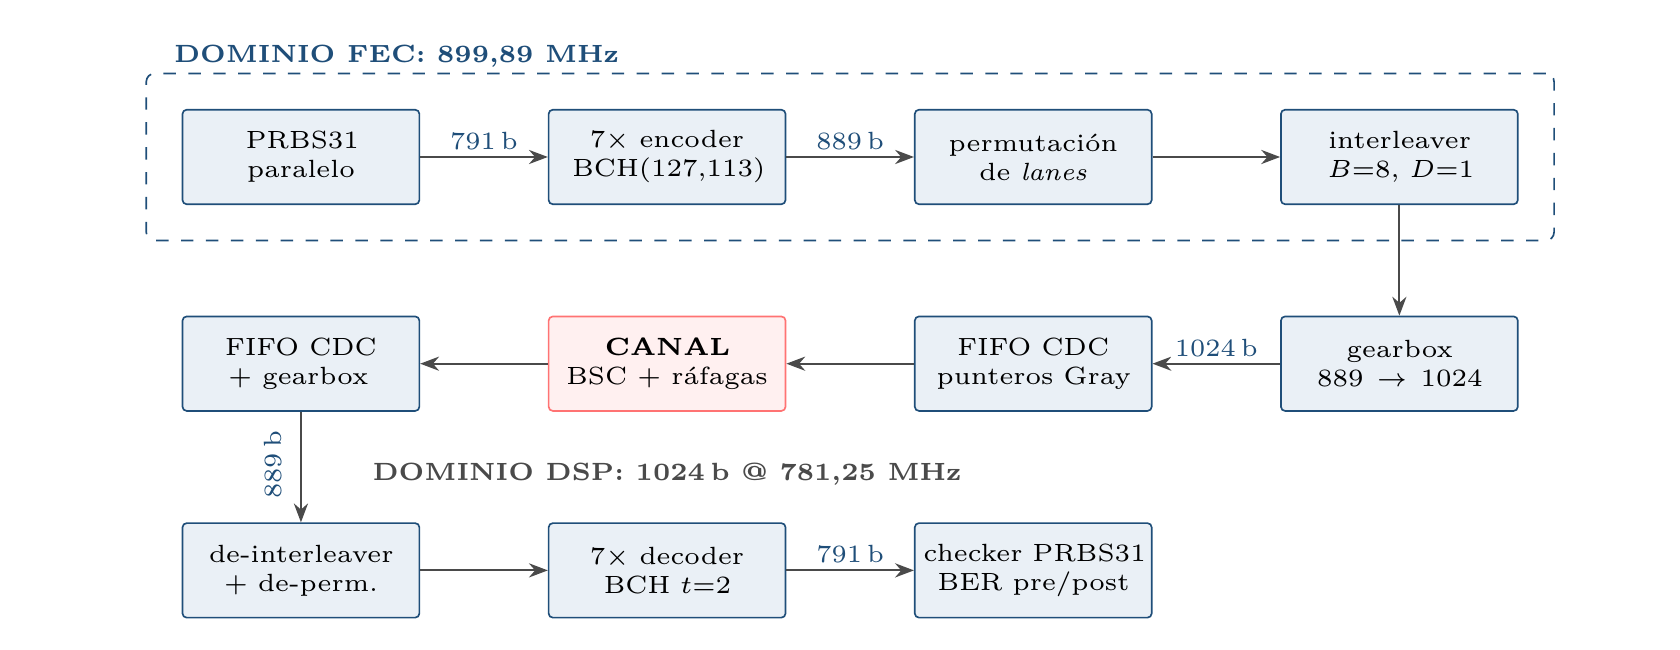
\includegraphics[width=\linewidth]{arquitectura_sistema.png}
    \caption{Cadena completa de transmisión, canal y recepción. El receptor
    replica el paralelismo del transmisor y las etiquetas indican los cambios de
    ancho de bus.}
    \label{fig:arquitectura}
\end{figure}


\subsubsection{Parámetros fijos}

La Tabla~\ref{tab:parametros-sistema} resume los parámetros fijos definidos por la especificación.

\begin{table}[H]
    \centering
    \caption{Parámetros principales de la cadena FEC.}
    \label{tab:parametros-sistema}
    \begin{tabular}{@{}lll@{}}
        \toprule
        \textbf{Parámetro} & \textbf{Valor} & \textbf{Observación}\\
        \midrule
        Código & BCH(127,113) & Primitivo, narrow-sense \\
        Campo de Galois & $\mathrm{GF}(2^7)$ & Polinomio primitivo $x^7+x^3+1$ \\
        Capacidad de corrección & $t=2$ & 14 bits de paridad\\
        Tasa del código & 113/127 = 0.8898 & \textit{overhead} 12.39\% \\
        Decisión & Dura(\textit{Hard}) & \\
        Encoders en paralelo & 7 &  \\
        Bus dominio FEC & 791 b entrada / 889 b salida & \\
        Frecuencia FEC  & $899,89$ MHz & Objetivo de síntesis: cerrar > 800MHz\\
        Bus dominio DSP & 1024 b &  \\
        Frecuencia DSP & 781,25 MHz & Ratio exacto 889:1024, gcd=1\\
        Tasa de línea & 800 Gb/s & Medida a la salida del DSP\\
        Tasa de payload & 711,811 Gb/s & \\
        Interleaver & Convolucional (Forney) & $B=8$, $D=1$ \\
        Secuencia de prueba & PRBS31: $x^{31} + x^{28} + 1$ &  \\
        \bottomrule
    \end{tabular}
\end{table}


\section{Desarrollo}

% ---------------------------------------------------------------------------
\subsection{Análisis y dimensionamiento del sistema}
\label{sec:etapa-0}

En esta primer etapa se hará un análisis del sistema en su totalidad, para determinar
las dimensiones y los detalles de cada etapa.
% ---------------------------------------------------------------------------

\subsubsection{Dimensionamiento del paralelismo y la tasa de datos}

La tasa codificada producida por $N$ codificadores BCH de longitud 127
operando en paralelo está dada por

\begin{equation}
    R_{\mathrm{linea}} = N\,127\,f_{\mathrm{FEC}}.
    \label{eq:tasa-linea}
\end{equation}

El dimensionamiento del paralelismo debe satisfacer simultáneamente la tasa
de línea requerida de $800$ Gb/s y la restricción sobre la frecuencia de
operación del dominio FEC.

Por lo tanto, para analizar las distintas alternativas de paralelismo, la
frecuencia necesaria para mantener la tasa de línea objetivo puede expresarse
como

\begin{equation}
    f_{\mathrm{FEC}}(N)
    =
    \frac{R_{\mathrm{linea}}}{127N}.
    \label{eq:fec-freq-N}
\end{equation}

Si se utilizaran únicamente seis codificadores en paralelo, la frecuencia
requerida sería

\begin{equation}
    f_{\mathrm{FEC}}(6)
    =
    \frac{800\text{ Gb/s}}{6\times127}
    =
    1{,}050\text{ GHz}.
\end{equation}

Si bien esta alternativa permite alcanzar la tasa de línea requerida, exige
superar $1$ GHz en el dominio FEC, lo que incrementaría considerablemente
la exigencia del cierre de timing.

Si, en cambio, se utilizaran ocho codificadores en paralelo, se obtendría

\begin{equation}
    f_{\mathrm{FEC}}(8)
    =
    \frac{800\text{ Gb/s}}{8\times127}
    =
    787{,}40\text{ MHz}.
\end{equation}

Aunque esta configuración también permite alcanzar los $800$ Gb/s mediante
un mayor grado de paralelismo, la frecuencia resultante queda por debajo de
los $800$ MHz establecidos como límite inferior para el dominio FEC.

Por lo tanto, $N=7$ es la configuración que satisface simultáneamente ambas
restricciones, resultando en una frecuencia de operación de

\begin{equation}
    f_{\mathrm{FEC}}
    =
    \frac{800\text{ Gb/s}}{7\times127}
    =
    899{,}89\text{ MHz}.
\end{equation}

Los siete codificadores producen en conjunto un bus codificado de

\begin{equation}
    W_{\mathrm{FEC}}
    =
    7\times127
    =
    889\text{ bits},
\end{equation}

mientras que el bus de información a la entrada tiene un ancho de

\begin{equation}
    W_{\mathrm{payload}}
    =
    7\times113
    =
    791\text{ bits}.
\end{equation}

Finalmente, debido a la tasa del código BCH$(127,113)$, la tasa de información
útil resulta

\begin{equation}
    R_{\mathrm{payload}}
    =
    800\text{ Gb/s}\frac{113}{127}
    =
    711{,}811\text{ Gb/s}.
    \label{eq:tasa-util}
\end{equation}

\subsubsection{Familia de códigos BCH}

Los códigos BCH forman una familia de códigos cíclicos cuya construcción parte
de especificar la capacidad de corrección deseada, en lugar de seleccionar
arbitrariamente un polinomio generador. Para un código BCH binario primitivo
\textit{narrow-sense} de longitud

\begin{equation}
    n = 2^m-1,
\end{equation}

se fija una capacidad de corrección diseñada $t$, asociada a una distancia
diseñada

\begin{equation}
    d_0 = 2t+1.
\end{equation}

A partir de este valor se exige que el polinomio generador tenga como raíces
las potencias consecutivas $\alpha,\alpha^2,\ldots,\alpha^{2t}$ de un elemento
primitivo $\alpha\in\mathrm{GF}(2^m)$. El polinomio generador resulta entonces

\begin{equation}
    g_t(x)
    =
    \operatorname{mcm}
    \left\{
        m_1(x),m_2(x),\ldots,m_{2t}(x)
    \right\},
    \label{eq:generador-bch-general}
\end{equation}

donde $m_i(x)$ es el polinomio mínimo de $\alpha^i$ sobre $\mathrm{GF}(2)$.
De esta forma,

\begin{equation}
    g_t(\alpha^i)=0,
    \qquad 1\leq i\leq2t,
\end{equation}

y la cota BCH garantiza que la distancia mínima real satisface

\begin{equation}
    d_{\min}\geq d_0=2t+1,
\end{equation}

permitiendo corregir, como mínimo, hasta $t$ errores por palabra de código.

La elección de las raíces no determina únicamente la capacidad de corrección,
sino también la redundancia del código. En efecto, las potencias conjugadas
por el automorfismo de Frobenius comparten un mismo polinomio mínimo. Los
exponentes correspondientes forman las clases ciclotómicas binarias

\begin{equation}
    C_i
    =
    \left\{
        i,2i,2^2i,\ldots
    \right\}
    \bmod n.
    \label{eq:clase-ciclotomica}
\end{equation}

Por lo tanto, al incluir una raíz $\alpha^i$ se incorporan automáticamente
todas las raíces cuyos exponentes pertenecen a la misma clase ciclotómica.
En consecuencia, cada polinomio mínimo asociado a una clase distinta aparece
una única vez en $g_t(x)$.

La dimensión $k$ del código queda determinada por el grado del polinomio
generador,

\begin{equation}
    k
    =
    n-\deg g_t(x)
    =
    n-
    \sum_{C_i\,\text{distintas}}
    \lvert C_i\rvert.
    \label{eq:dimension-bch-cosets}
\end{equation}

Esta relación muestra que, una vez fijados $n$ y $t$, la dimensión $k$ no
constituye un parámetro independiente, sino que resulta de las clases
ciclotómicas alcanzadas por las raíces consecutivas utilizadas en la
construcción del código.

En este trabajo se utiliza $m=7$, por lo que

\begin{equation}
    n=2^7-1=127.
\end{equation}

Como el orden multiplicativo de $2$ módulo $127$ es $7$, todas las clases
ciclotómicas no nulas tienen siete elementos. En consecuencia, cada nueva
clase incorporada al polinomio generador aumenta su grado en siete y agrega
siete bits de redundancia.

La Tabla~\ref{tab:familia-bch-127} muestra los códigos obtenidos al variar la
capacidad de corrección diseñada $t$.

\begin{table}[H]
    \centering
    \small
    \caption{Familia BCH binaria primitiva \textit{narrow-sense} de longitud 127.}
    \label{tab:familia-bch-127}
    \begin{tabular}{@{}c c c p{7.0cm} c@{}}
        \toprule
        $t$ & $k$ & $n-k$ & Clases ciclotómicas utilizadas & $k/n$ \\
        \midrule
         1 & 120 &  7 & $C_1$ & 0,9449 \\
         2 & 113 & 14 & $C_1,C_3$ & 0,8898 \\
         3 & 106 & 21 & $C_1,C_3,C_5$ & 0,8346 \\
         4 &  99 & 28 & $C_1,C_3,C_5,C_7$ & 0,7795 \\
         5 &  92 & 35 & $C_1,C_3,C_5,C_7,C_9$ & 0,7244 \\
         6 &  85 & 42 & $C_1,C_3,C_5,C_7,C_9,C_{11}$ & 0,6693 \\
         7 &  78 & 49 & $C_1,C_3,C_5,C_7,C_9,C_{11},C_{13}$ & 0,6142 \\
         8 &  71 & 56 & $C_1,C_3,C_5,C_7,C_9,C_{11},C_{13},C_{15}$ & 0,5591 \\
         9 &  71 & 56 & $C_1,C_3,C_5,C_7,C_9,C_{11},C_{13},C_{15}$ & 0,5591 \\
        10 &  64 & 63 & $C_1,C_3,C_5,C_7,C_9,C_{11},C_{13},C_{15},C_{19}$ & 0,5039 \\
        \bottomrule
    \end{tabular}
\end{table}

En particular, para $t=2$ deben incluirse las raíces
$\alpha^1,\alpha^2,\alpha^3$ y $\alpha^4$. Las raíces $\alpha^1$,
$\alpha^2$ y $\alpha^4$ pertenecen a $C_1$, mientras que $\alpha^3$
pertenece a $C_3$. Por lo tanto,

\begin{equation}
    g(x)=\operatorname{mcm}\{m_1(x),m_2(x),m_3(x),m_4(x)\}
        =m_1(x)m_3(x),
\end{equation}

y, dado que ambas clases tienen siete elementos,

\begin{equation}
    \deg g(x)=7+7=14,
\end{equation}

de donde resulta

\begin{equation}
    k=127-14=113.
\end{equation}

De esta manera se verifica que el código BCH$(127,113)$ especificado es un
miembro realizable de la familia y corresponde a una capacidad de corrección
diseñada de $t=2$ errores por palabra.

Los restantes valores de $t$ de la tabla también dan lugar a códigos BCH
válidos de longitud 127, con distintos compromisos entre capacidad de
corrección y tasa de código. Incrementar $t$ aumenta la protección frente a
errores, pero en general requiere incorporar nuevas clases ciclotómicas,
aumentando la redundancia y reduciendo la tasa de información útil
transmitida.

La elección de $t$ constituye, por lo tanto, una decisión de diseño que debe
realizarse a partir de las características del canal y de los requisitos de
desempeño del sistema, considerando, entre otros aspectos, la estadística de
errores esperada y la tasa de error admisible después de la decodificación.
Para la arquitectura desarrollada en este trabajo se adopta el valor
especificado $t=2$ y, en consecuencia, el código BCH$(127,113)$.

\subsubsection{Construcción del código BCH(127,113)}

A partir de la construcción general presentada anteriormente, se particulariza
ahora el caso correspondiente al código BCH$(127,113)$ utilizado en el sistema.
Para $m=7$, la longitud de un código BCH binario primitivo viene dada por

\begin{equation}
    n=2^m-1=127.
\end{equation}

El código especificado posee capacidad de corrección diseñada $t=2$, por lo que
su distancia diseñada es

\begin{equation}
    d_0=2t+1=5.
\end{equation}

Al tratarse de un código BCH primitivo \textit{narrow-sense}, el polinomio
generador debe tener como raíces consecutivas a

\begin{equation}
    \alpha^1,\alpha^2,\alpha^3,\alpha^4,
\end{equation}

donde $\alpha$ es un elemento primitivo de $\mathrm{GF}(2^7)$. Como se explicó
anteriormente, las raíces conjugadas pertenecientes a una misma clase ciclotómica
comparten el mismo polinomio mínimo. Para este caso, las potencias involucradas
quedan contenidas en las clases

\begin{align}
    C_1 &= \{1,2,4,8,16,32,64\}, \\
    C_3 &= \{3,6,12,24,48,96,65\}.
\end{align}

En particular, $\alpha^1$, $\alpha^2$ y $\alpha^4$ pertenecen a $C_1$, mientras
que $\alpha^3$ pertenece a $C_3$. Por lo tanto, sólo es necesario incorporar los
polinomios mínimos asociados a estas dos clases.

Utilizando el polinomio primitivo adoptado para la construcción de
$\mathrm{GF}(2^7)$, los polinomios mínimos correspondientes son

\begin{align}
    m_1(x) &= x^7+x^3+1, \\
    m_3(x) &= x^7+x^3+x^2+x+1.
\end{align}

El polinomio generador del código resulta entonces del mínimo común múltiplo
de los polinomios mínimos asociados a las raíces requeridas. Dado que
$m_1(x)$ y $m_3(x)$ son distintos e irreducibles sobre $\mathrm{GF}(2)$,

\begin{equation}
    g(x)
    =
    \operatorname{mcm}
    \left\{
        m_1(x),m_3(x)
    \right\}
    =
    m_1(x)m_3(x).
\end{equation}

Desarrollando el producto se obtiene

\begin{equation}
\begin{split}
    g(x)
    &=
    \left(x^7+x^3+1\right)
    \left(x^7+x^3+x^2+x+1\right) \\
    &=
    x^{14}+x^9+x^8+x^6+x^5+x^4+x^2+x+1.
\end{split}
\label{eq:polinomio-generador}
\end{equation}

El grado del polinomio generador es, por lo tanto,

\begin{equation}
    \deg g(x)=14.
\end{equation}

Como en un código cíclico la redundancia es igual al grado de $g(x)$, se
obtiene

\begin{equation}
    n-k=\deg g(x)=14,
\end{equation}

y, en consecuencia,

\begin{equation}
    k=n-\deg g(x)=127-14=113.
\end{equation}

De esta manera queda verificada la construcción del código BCH$(127,113)$
especificado. Cada palabra de información de 113 bits se codifica en una
palabra de 127 bits mediante la incorporación de 14 bits de redundancia, y la
cota BCH garantiza una distancia mínima

\begin{equation}
    d_{\min}\geq5,
\end{equation}

suficiente para corregir hasta dos errores por palabra de código.

La tabla completa de elementos de $\mathrm{GF}(2^7)$ utilizada para esta
construcción se presenta en la Tabla~\ref{tab:elementos-gf27} del
Anexo~\ref{anexo:elementos-gf27}. Allí se incluyen las potencias de $\alpha$ y
sus representaciones polinómica y binaria, lo que permite verificar las
relaciones entre los elementos del campo, las clases ciclotómicas empleadas y
los polinomios mínimos obtenidos.

\subsubsection{Dimensionamiento del gearbox y la FIFO}

El cambio entre el dominio FEC y el dominio DSP requiere adaptar tanto el ancho
de palabra como la frecuencia de operación. El dominio FEC entrega palabras de
889 bits a $f_{\mathrm{FEC}}=899{,}89$ MHz, mientras que el dominio DSP procesa
palabras de 1024 bits a $f_{\mathrm{DSP}}=781{,}25$ MHz. Aunque ambos dominios
transportan la misma tasa media de $800$ Gb/s, la conversión entre anchos genera
un patrón de transferencias no uniforme que debe ser tenido en cuenta para
dimensionar correctamente el gearbox y la FIFO CDC.

El gearbox recibe 889 bits en cada ciclo FEC y acumula los datos hasta disponer
de una palabra completa de 1024 bits para escribir en la FIFO. Luego de $n$
ciclos FEC, la cantidad acumulada de palabras completas y el número de bits que
permanecen almacenados internamente en el gearbox pueden expresarse 
correspondientemente como

\begin{align}
    W(n)
    &=
    \left\lfloor
        \frac{889n}{1024}
    \right\rfloor,
    \label{eq:gearbox-palabras}
    \\
    r(n)
    &=
    889n \bmod 1024.
    \label{eq:gearbox-residuo}
\end{align}

El estado interno del gearbox se repite cuando el residuo vuelve a cero. Como 
$\gcd(889,1024)=1$, es decir son coprimos, el menor valor de $n\neq0$ para el 
cual se cumple $r(n)=0$ es $n=1024$

Durante estos 1024 ciclos FEC ingresan exactamente 889 palabras de 1024 bits. 
Por lo tanto, un período completo del patrón del gearbox comprende 1024 
ciclos FEC y genera 889 transferencias hacia la FIFO.

Este resultado es consistente con la relación entre las frecuencias de ambos
dominios,

\begin{equation}
    \frac{f_{\mathrm{DSP}}}{f_{\mathrm{FEC}}}
    =
    \frac{889}{1024},
    \qquad
    889f_{\mathrm{FEC}}
    =
    1024f_{\mathrm{DSP}}
    =
    800\text{ Gb/s}.
    \label{eq:relacion-clocks-gearbox}
\end{equation}

Sin embargo, la igualdad de tasas medias no implica que el gearbox produzca
una nueva palabra en cada ciclo FEC. Para describir el patrón instantáneo de
escrituras se define

\begin{equation}
    \Delta W(n)=W(n)-W(n-1),
    \label{eq:gearbox-write-valid}
\end{equation}

donde $\Delta W(n)=1$ indica que durante el ciclo $n$ se completó una nueva
palabra de 1024 bits, mientras que $\Delta W(n)=0$ representa un ciclo sin
escritura hacia la FIFO.

Como en un período completo existen 1024 ciclos FEC y sólo se generan 889
palabras, el número total de ciclos sin escritura resulta

\begin{equation}
    N_{\mathrm{gap}}
    =
    1024-889
    =
    135.
    \label{eq:gearbox-gaps}
\end{equation}

La Tabla~\ref{tab:gearbox-primer-gap} muestra la evolución inicial del gearbox
hasta el primer ciclo sin salida posterior al llenado inicial.

\begin{table}[H]
    \centering
    \caption{Evolución inicial del gearbox hasta el primer hueco no inicial.}
    \label{tab:gearbox-primer-gap}
    \begin{tabular}{@{}rrrrl@{}}
        \toprule
        Ciclo FEC $n$ & Bits ingresados & $W(n)$ & $r(n)$ & $\Delta W(n)$ \\
        \midrule
        1 &  889 & 0 & 889 & 0 \\
        2 & 1778 & 1 & 754 & 1 \\
        3 & 2667 & 2 & 619 & 1 \\
        4 & 3556 & 3 & 484 & 1 \\
        5 & 4445 & 4 & 349 & 1 \\
        6 & 5334 & 5 & 214 & 1 \\
        7 & 6223 & 6 &  79 & 1 \\
        8 & 7112 & 6 & 968 & 0 \\
        \bottomrule
    \end{tabular}
\end{table}

El primer ciclo corresponde a la latencia inevitable de llenado del gearbox.
Sin embargo, en el ciclo 8 aparece un nuevo ciclo sin escritura aun cuando la
producción de palabras ya se encuentra en régimen. Este comportamiento se repite
a lo largo de todo el período de 1024 ciclos.

La FIFO desacopla este patrón irregular de escrituras del patrón de lecturas del
dominio DSP. Para analizar su comportamiento se define la ocupación física como

\begin{equation}
    Q(t)
    =
    N_W(t)-N_R(t),
    \label{eq:fifo-ocupacion}
\end{equation}

donde $N_W(t)$ y $N_R(t)$ representan, respectivamente, la cantidad acumulada
de escrituras y lecturas hasta el instante $t$. Para evitar condiciones de
underflow y overflow debe cumplirse

\begin{equation}
    0\leq Q(t)\leq D,
    \label{eq:fifo-limites-ocupacion}
\end{equation}

siendo $D$ la profundidad de la FIFO.

A pesar de que las tasas medias de escritura y lectura son idénticas, los
eventos instantáneos no se encuentran necesariamente alineados. Durante un
período completo ocurren 1024 flancos FEC y 889 flancos DSP. Por lo tanto,
existen 135 ciclos menos en el dominio DSP, exactamente la misma cantidad de
ciclos FEC en los que el gearbox no genera una nueva palabra.

Además, la relación de fase entre ambos relojes es desconocida, por lo que una
determinada fase puede hacer que un flanco de lectura ocurra antes de que el 
gearbox  haya escrito la siguiente palabra. Si la lectura comenzara apenas 
estuviese disponible la primera palabra, esta diferencia temporal podría 
agotar transitoriamente las palabras en la FIFO.

Si bien el mecanismo de la propia FIFO impediría una lectura físicamente 
inválida, dicho ciclo no realizaría una transferencia y reduciría la tasa de 
transferencia de línea. Por este motivo es necesario incorporar un nivel de 
arranque, de forma que el dominio DSP permanezca en pausa hasta observar 
una cantidad mínima de palabras disponibles en la FIFO.

El análisis debe considerar además la latencia propia del cruce de dominio 
de los punteros de lectura y escritura de la FIFO. Por ejemplo, el puntero 
de escritura se genera en el dominio FEC y atraviesa un sincronizador de 
dos etapas antes de ser utilizado por la lógica del dominio DSP.

Como consecuencia, debe distinguirse entre la ocupación física de la memoria y
la ocupación observada desde el dominio lector. Durante los transitorios puede
ocurrir que

\begin{equation}
    Q_{\mathrm{visible,DSP}}(t)
    \neq
    Q_{\mathrm{real}}(t),
\end{equation}

ya que una palabra físicamente escrita puede requerir hasta dos flancos DSP
adicionales para verse reflejada en el puntero de escritura sincronizado. Este
comportamiento es conservador desde el punto de vista funcional, dado que el
lector nunca puede acceder a información que todavía no haya sido escrita. Sin
embargo, retrasa el conocimiento de las nuevas escrituras y aumenta el margen
de ocupación necesario durante el arranque.

Para verificar el comportamiento conjunto del gearbox, la FIFO y los
sincronizadores se implementó un modelo temporal en Python. Los períodos de
reloj se expresaron utilizando una unidad de tiempo entera,

\begin{equation}
    T_{\mathrm{FEC}}=889,
    \qquad
    T_{\mathrm{DSP}}=1024.
\end{equation}

De esta manera se conserva exactamente la relación requerida,

\begin{equation}
    \frac{T_{\mathrm{DSP}}}{T_{\mathrm{FEC}}}
    =
    \frac{1024}{889},
\end{equation}

y, dado que ambos períodos son coprimos, los relojes vuelven a presentar la
misma relación de fase luego del superperíodo

\begin{equation}
    T_{\mathrm{super}}
    =
    \operatorname{mcm}(889,1024)
    =
    889\times1024.
    \label{eq:superperiodo-fifo}
\end{equation}

Durante este intervalo ocurren exactamente 1024 ciclos FEC y 889 ciclos DSP, por
lo que también se recorre un período completo del patrón del gearbox.

Tomando como referencia un flanco FEC en $t=0$, el primer flanco DSP puede
ubicarse en cualquiera de las 1024 posiciones enteras dentro de su período, 
pudiendo analizar las 1024 fases iniciales posibles del dominio DSP para
cada nivel de arranque considerado.

El modelo reproduce la acumulación de bits del gearbox, las escrituras y lecturas
de la FIFO y los sincronizadores de punteros.
Una fase se considera fallida si, una vez habilitada la lectura, aparece al menos
un ciclo DSP sin una palabra visible o si se produce un overflow.

Para el análisis se adoptó inicialmente una FIFO de profundidad 8. La elección de
una profundidad potencia de dos resulta conveniente para la implementación de los
punteros binarios y Gray de una FIFO asíncrona, y proporciona además margen para
evaluar distintos niveles de arranque. La
configuración utilizada se resume en la Tabla~\ref{tab:fifo-configuracion}.

\begin{table}[H]
    \centering
    \caption{Configuración utilizada para dimensionar la FIFO CDC.}
    \label{tab:fifo-configuracion}
    \begin{tabular}{@{}lr@{}}
        \toprule
        Parámetro & Valor \\
        \midrule
        Ancho & 1024 bits \\
        Etapas de sincronización & 2 \\
        Profundidad evaluada & 8 palabras \\
        Umbrales de arranque analizados & 1 a 4 palabras \\
        Fases iniciales analizadas & 1024 \\
        \bottomrule
    \end{tabular}
\end{table}

Los resultados del barrido se presentan en la
Tabla~\ref{tab:fifo-barrido}.

\begin{table}[H]
    \centering
    \caption{Barrido del umbral de arranque para una FIFO de ocho palabras.}
    \label{tab:fifo-barrido}
    \begin{tabular}{@{}rrrrr@{}}
        \toprule
        Umbral & Fases fallidas & Huecos & Overflow & Ocup. máxima \\
        \midrule
        1 & 134 & 134 & 0 & 3 \\
        2 &   0 &   0 & 0 & 4 \\
        3 &   0 &   0 & 0 & 5 \\
        4 &   0 &   0 & 0 & 6 \\
        \bottomrule
    \end{tabular}
\end{table}

El barrido muestra que un nivel de arranque de una sola palabra no constituye
un margen suficiente ya que 134 de las 1024 relaciones de fase analizadas producen al
menos un hueco luego de habilitar la lectura. En cambio, un nivel de dos palabras
evita underflow y overflow para todas las fases simuladas. Por lo tanto, para el
modelo nominal se obtiene

\begin{equation}
    \texttt{START\_LEVEL}_{\min}=2.
\end{equation}

Este valor representa el mínimo funcional determinado por el barrido, pero para 
proporcionar un margen adicional frente a escenarios reales no modelados, se 
selecciona

\begin{equation}
    \texttt{START\_LEVEL}=4.
\end{equation}

Con este valor, la ocupación máxima observada durante el barrido es de seis
palabras. Una profundidad de ocho posiciones conserva, por lo tanto, dos entradas
libres respecto del máximo alcanzado en el caso nominal.

Como el productor y el consumidor transportan exactamente la misma tasa media,
en condiciones normales de funcionamiento la ocupación no presenta una deriva
creciente. El barrido de todas las fases relativas confirma este comportamiento:
para el nivel de arranque seleccionado no se observa overflow y la ocupación
permanece acotada a seis palabras. La profundidad de ocho palabras deja así un
margen de dos posiciones respecto de la máxima ocupación observada, por lo que la
FIFO no opera cerca de su capacidad máxima en el funcionamiento nominal.

La configuración final adoptada para el cruce entre los dominios FEC y DSP es

\begin{equation}
    \boxed{
    \begin{aligned}
        D &= 8\text{ palabras},\\
        W_{\mathrm{FIFO}} &= 1024\text{ bits},\\
        N_{\mathrm{sync}} &= 2,\\
        \texttt{START\_LEVEL} &= 4.
    \end{aligned}}
    \label{eq:fifo-configuracion-final}
\end{equation}

El barrido temporal demuestra que esta configuración evita underflow y overflow
para todas las relaciones de fase analizadas, al mismo tiempo que mantiene un
margen adicional respecto del mínimo funcional obtenido para el caso nominal.

\subsubsection{Análisis del sistema de entrelazado}

El sistema utiliza dos mecanismos consecutivos de entrelazado con el objetivo
de aumentar la tolerancia frente a errores en ráfaga de duración prolongada. 
En primer lugar, la permutación de lanes intercala bit a bit las siete 
codewords BCH generadas en paralelo. En segundo lugar, un interleaver 
convolucional de Forney distribuye las posiciones resultantes entre ocho 
ramas con retardos temporales escalonados.

El interleaver no introduce capacidad de corrección adicional. Su función es
redistribuir temporal y espacialmente los errores de manera que, luego del
de-interleaver, cada codeword BCH reciba una cantidad de errores compatible
con su capacidad de corrección $t=2$.

\paragraph{Combinación de la permutación de lanes y el interleaver}

Como determina la especificación , dada ciclo del dominio FEC produce 
siete codewords en paralelo, una por cada encoder BCH. Una concatenación 
directa dejaría 127 bits consecutivos pertenecientes a la misma codeword 
y quedaría vulnerable a rafagas de errores. Para evitar esto, se utiliza 
la permutación de lanes que intercala los siete codewords bit a bit. 
Primero ubica el bit $j$ de todos los codewords y recién después 
continúa con el bit $j+1$:

\begin{equation}
    \operatorname{linea}[7j+\ell]
    =
    \mathrm{CW}_{\ell}[j],
    \qquad
    0\leq \ell<7,
    \quad
    0\leq j<127.
    \label{eq:permutacion-lanes-p4}
\end{equation}

\begin{figure}[H]
    \centering
    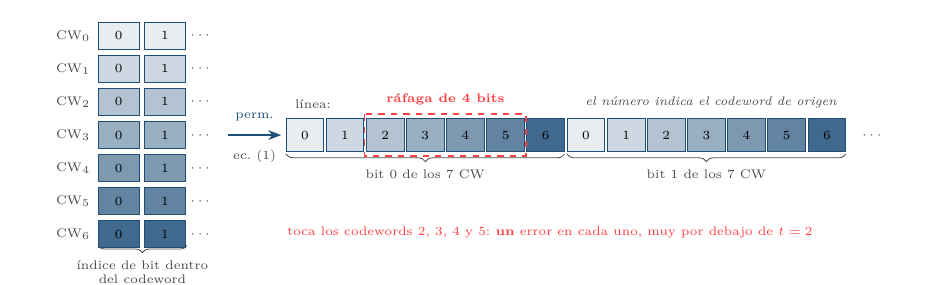
\includegraphics[width=0.98\textwidth]{permutacion_lanes.png}
    \caption{Permutación de lanes. Una ráfaga corta toca bits de codewords
    diferentes en lugar de concentrarse sobre uno solo.}
    \label{fig:permutacion-lanes}
\end{figure}

Como se observa en la Fig.~\ref{fig:permutacion-lanes}, una ráfaga de cuatro
bits consecutivos afecta a cuatro codewords distintas, con un error en cada una.
Cada decodificador recibe así un único error, muy por debajo de su capacidad
$t=2$. En general, si $p$ representa una posición dentro del frame, la codeword
de origen queda determinada por

\begin{equation}
    c(p)=p\bmod 7.
    \label{eq:codeword-posicion-p4}
\end{equation}

De esta forma, 2 bits consecutivos pertenecen a codewords distintas y una misma
codeword reaparece cada siete posiciones.

Si bien la permutación de lanes protege contra ráfagas cortas, su alcance está
limitado por los siete codewords disponibles en paralelo. Para proteger frente
a ráfagas más largas es necesario separar los bits también a lo largo del
tiempo. Para ello se incorpora en conjunto el interleaver convolucional de Forney. 
Su mecanismo de funcionamiento es que las posiciones del frame se distribuyen 
cíclicamente entre $B$ ramas y cada rama introduce un retardo distinto, 
múltiplo de $D$:

\begin{equation}
    \operatorname{rama}(p)=p\bmod B,
    \qquad
    \operatorname{retardo}_{\mathrm{TX}}(p)=(p\bmod B)D.
    \label{eq:rama-posicion-p4}
\end{equation}

La rama 0 pasa directamente, la rama 1 se retrasa $D$ ciclos, la rama 2 se
retrasa $2D$ ciclos y así sucesivamente hasta la rama $B-1$, que se retrasa
$(B-1)D$ ciclos. Para $B=8$ y $D=1$, los retardos del transmisor son

\begin{equation}
    0,1,2,\ldots,7\text{ ciclos FEC}.
\end{equation}

El resultado es que bits que ingresaron juntos al interleaver salen escalonados
en el tiempo. El receptor debe deshacer ese escalonamiento y, para ello, el
de-interleaver aplica a cada posición el retardo complementario

\begin{equation}
    \operatorname{retardo}_{\mathrm{RX}}(p)
    =\left(B-1-(p\bmod B)\right)D.
    \label{eq:retardo-rx-forney}
\end{equation}

\begin{figure}[H]
    \centering
    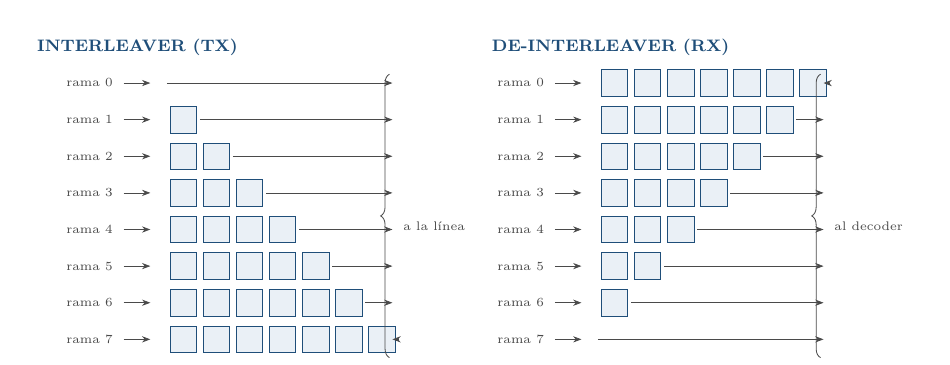
\includegraphics[width=0.90\textwidth]{interleaver_forney.png}
    \caption{Interleaver convolucional de Forney y de-interleaver con retardos
    complementarios.}
    \label{fig:interleaver-forney}
\end{figure}

Al sumar los retardos del transmisor y del receptor, un bit ubicado en la rama
$b=p\bmod B$ acumula

\begin{equation}
    bD+(B-1-b)D=(B-1)D.
\end{equation}

La latencia conjunta es independiente de la posición del bit. Esta es la
propiedad que permite recuperar el alineamiento de los codewords sin incorporar
lógica adicional de realineado. Con $B=8$ y $D=1$, todos los bits acumulan siete
ciclos FEC entre el interleaver y el de-interleaver.

La ventaja principal de combinar la permutación de lanes con el interleaver
surge de la relación aritmética entre sus períodos. Dentro de un mismo frame,
los bits de una misma codeword reaparecen cada 7 posiciones de línea, mientras
que una misma rama del interleaver reaparece cada 8 posiciones. Por lo tanto,
para que dos errores queden asociados nuevamente a la misma codeword y además
atraviesen la misma rama de retardo, su separación $d$ debe ser múltiplo
simultáneamente de 7 y de 8. Como 7 y 8 son coprimos, la menor separación que
cumple ambas condiciones es

\begin{equation}
    P_{\mathrm{par}}
    =
    \operatorname{mcm}(7,8)
    =
    56.
    \label{eq:periodo-pareja-lane-rama}
\end{equation}

Por lo tanto, la misma combinación $(\text{codeword},\text{rama})$ solamente
vuelve a aparecer cada 56 posiciones de línea. Mientras que la permutación de
lanes por sí sola haría reaparecer una misma codeword cada siete posiciones,
las sucesivas apariciones de la codeword recorren las ocho ramas del interleaver
antes de volver a experimentar el mismo retardo.

Para una combinación determinada, las posiciones potencialmente asociadas a
una misma codeword después del de-interleaver presentan entonces la secuencia

\begin{equation}
    p_0,\quad
    p_0+56,\quad
    p_0+112,\quad\ldots
    \label{eq:posiciones-mismo-codeword-p4}
\end{equation}

El BCH utilizado puede corregir hasta $t=2$ errores dentro de una misma
palabra. Una ráfaga de longitud $L=112$ comprende posiciones desde $p_0$ hasta
$p_0+111$, por lo que puede contener como máximo dos elementos de la secuencia
anterior. Ambos errores permanecen dentro de la capacidad de corrección del
código.

Por lo tanto, para una ráfaga completamente contenida dentro de un frame,

\begin{equation}
    L_{\max,\mathrm{frame}}
    =
    t\,\operatorname{mcm}(7,8)
    =
    2\cdot56
    =
    112\text{ bits}.
    \label{eq:rafaga-maxima-p4}
\end{equation}

Una ráfaga de 113 bits de errores constituye la primera longitud potencialmente 
incorregible. Esto no implica que toda ráfaga de 113 bits produzca necesariamente 
un error de decodificación, sino que deja de existir garantía de corrección 
para cualquier offset de inicio.

\paragraph{Efecto del cruce entre frames consecutivos}

El análisis anterior supone que la ráfaga de errores se encuentra completamente 
contenida dentro de un frame de 889 bits. Sin embargo, el interleaver determina 
la rama a partir de la posición local $p$ dentro de cada frame. Como

\begin{equation}
    889\bmod8=1,
    \label{eq:frame-mod-b}
\end{equation}

el ancho del frame no coincide con un número entero de períodos de las 8
ramas. Por este motivo, al finalizar un frame y reiniciar la numeración local
en $p=0$, la secuencia de ramas no continúa de forma periódica a través del
borde.

Este efecto puede observarse en las últimas posiciones de un frame y las
primeras del siguiente, como se indica en la Tabla \ref{tab:borde-frames}.

\begin{table}[H]
\centering
\begin{tabular}{c|ccc|ccc}
\textbf{Frame} & \multicolumn{3}{c|}{\textbf{Frame $n$}}
               & \multicolumn{3}{c}{\textbf{Frame $n+1$}} \\
\hline
Posición local $p$ & 886 & 887 & 888 & 0 & 1 & 2 \\
\hline
Rama $b(p)=p\bmod 8$ & 6 & 7 & 0 & 0 & 1 & 2
\end{tabular}
\caption{Asignación de ramas alrededor del borde entre dos frames consecutivos.}
\label{tab:borde-frames}
\end{table}

Para estudiar el efecto que tiene sobre una ráfaga de errores, considérese una 
posición $p_1$ del frame de salida $n$ y una posición $p_2$ del frame de salida 
$n+1$. Debido al interleaver, un bit observado en el frame $n$ que pertenece a 
la rama $b$ se originó $b$ ciclos antes. Por lo tanto, su índice temporal previo 
al interleaver puede expresarse como

\begin{equation}
    n_{\mathrm{orig}}=n-b.
    \label{eq:frame-original}
\end{equation}

Para que dos errores ubicados en frames consecutivos terminen asociados a la
misma instancia temporal después del de-interleaver debe cumplirse

\begin{equation}
    n-b(p_1)
    =
    (n+1)-b(p_2).
\end{equation}

De aquí se obtiene

\begin{equation}
    b(p_2)=b(p_1)+1.
    \label{eq:rama-borde}
\end{equation}

Es decir, al avanzar un frame en el tiempo, la segunda posición del error debe
atravesar una rama cuyo retardo sea un ciclo mayor para que ambos bits vuelvan
a alinearse sobre la misma palabra original.

Sea $d$ la separación entre ambos errores medida sobre la línea. Si se cruza
un único borde de frame,

\begin{equation}
    p_2=p_1+d-889.
    \label{eq:posicion-despues-borde}
\end{equation}

La condición de ramas requiere

\begin{equation}
    p_2
    \equiv
    p_1+1
    \pmod 8.
\end{equation}

Sustituyendo la Ec.~\eqref{eq:posicion-despues-borde},

\begin{equation}
    p_1+d-889
    \equiv
    p_1+1
    \pmod 8.
\end{equation}

Como $889\equiv1\pmod8$, resulta

\begin{equation}
    d\equiv2\pmod8.
    \label{eq:condicion-rama-borde}
\end{equation}

Simultáneamente, para que ambos errores correspondan a la misma codeword BCH,
la separación debe cumplir

\begin{equation}
    d\equiv0\pmod7.
    \label{eq:condicion-lane-borde}
\end{equation}

Por lo tanto, la separación $d$ debe satisfacer simultáneamente

\begin{equation}
    d\equiv0\pmod7
    \qquad\land\qquad
    d\equiv2\pmod8.
\end{equation}

La menor solución positiva de este sistema es

\begin{equation}
    d_{\mathrm{borde}}=42.
    \label{eq:distancia-borde}
\end{equation}

Como ejemplo, considérese la posición $p_1=882$ de un frame y la posición
$p_2=35$ del frame siguiente. La distancia entre ambas sobre la línea es

\begin{equation}
    d=(889-882)+35=42.
\end{equation}

Ambas posiciones corresponden al mismo lane,

\begin{equation}
    882\bmod7
    =
    35\bmod7
    =
    0,
\end{equation}

mientras que sus ramas son

\begin{equation}
    882\bmod8=2,
    \qquad
    35\bmod8=3.
\end{equation}

El segundo error aparece un ciclo FEC más tarde pero atraviesa también una
rama con un ciclo adicional de retardo. Como consecuencia, ambos errores
pueden terminar asociados a la misma codeword después del de-interleaver.

Este efecto reduce la separación mínima respecto del caso completamente
contenido dentro de un frame. En el peor alineamiento, tres errores que
terminan afectando a la misma codeword pueden aparecer con una separación de
56 posiciones entre los dos primeros y de 42 posiciones entre el segundo y el
tercero. La distancia entre el primer y el tercer error resulta entonces

\begin{equation}
    d_{\mathrm{3err}}
    =
    56+42
    =
    98.
    \label{eq:span-tres-errores-borde}
\end{equation}

Por lo tanto, al considerar todos los offsets posibles, incluidos aquellos que
cruzan el borde entre frames, la longitud máxima garantizadamente corregible
se reduce a

\begin{equation}
    L_{\max,\mathrm{global}}
    =
    98\text{ bits}.
    \label{eq:rafaga-maxima-global}
\end{equation}

La primera longitud potencialmente no corregible pasa a ser entonces 99 bits.

Este análisis demuestra que una evaluación restringida a ráfagas que no
atraviesen el borde entre frames produciría el resultado optimista de
112 bits. Al considerar también los offsets que cruzan el borde, la longitud
máxima de ráfaga garantizadamente corregible se reduce a 98 bits, es decir,
14 bits menos que en el caso contenido dentro de un único frame.


\paragraph{Modificación para recuperar la protección completa}

La pérdida de protección observada en el cruce entre frames se origina porque
la asignación de ramas se reinicia en cada nuevo frame a partir de la posición
local $p=0$. Como $889\bmod8=1$, la secuencia global de ramas debería avanzar
una posición entre frames consecutivos para mantener la periodicidad natural del
interleaver.

Una forma de recuperar esta propiedad consiste en introducir una fase de
interleaving $\phi_n$ asociada al frame $n$, definida como

\begin{equation}
    \phi_{n+1}
    =
    (\phi_n+1)\bmod8.
\end{equation}

La asignación de ramas dejaría entonces de depender únicamente de la posición
local y pasaría a definirse como

\begin{equation}
    b_n(p)
    =
    (p+\phi_n)\bmod8.
\end{equation}

De esta manera, cada nuevo frame comienza el interleaving desplazado una rama
respecto del anterior. En lugar de reiniciar siempre con la secuencia
$0,1,\ldots,7$, los frames consecutivos comenzarían con fases
$0,1,2,\ldots,7$ y luego volverían a cero. Esto permite que la asignación de
ramas sea equivalente a la obtenida sobre una numeración global continua de
los bits de línea.

Desde el punto de vista RTL, los bits pueden agruparse inicialmente de forma
estática según su posición local módulo 8,

\begin{equation}
    G_i=\{p:\ p\bmod8=i\},
\end{equation}

y posteriormente aplicar una rotación cíclica entre estos ocho grupos y las
ocho ramas físicas del interleaver. La fase $\phi_n$, representada mediante un
contador módulo 8, controlaría esta multiplexación. Por ejemplo, para
$\phi_n=1$, el grupo $G_0$ se conecta a la rama 1, $G_1$ a la rama 2 y así
sucesivamente hasta conectar $G_7$ a la rama 0.

Esta modificación elimina la discontinuidad introducida por el borde de frame
y recupera la periodicidad conjunta determinada por
$\operatorname{mcm}(7,8)=56$. En consecuencia, la longitud máxima de ráfaga
garantizadamente corregible vuelve al valor de 112 bits obtenido para una
ráfaga contenida completamente dentro de un frame.

El costo de esta solución se encuentra principalmente en la red de
multiplexación necesaria para realizar la rotación dinámica de los ocho grupos.
A diferencia de la implementación original, donde la asignación de posiciones
a ramas es estática y puede resolverse esencialmente mediante cableado, la
versión con fase variable requiere lógica combinacional adicional sobre un
datapath de 889 bits. A simple vista, esto implica un aumento significativo de
área y la incorporación de nuevos multiplexores en el camino crítico del
dominio FEC, que debe operar a una frecuencia cercana a $900\,\mathrm{MHz}$.

Por lo tanto, la modificación presenta un compromiso claro entre protección y
costo de implementación. Se recuperan 14 bits de longitud máxima de ráfaga,
pasando de 98 a 112 bits, pero a cambio de una red de multiplexación de ancho
elevado y una mayor exigencia sobre el cierre de timing. Dado que la mejora en
protección es relativamente pequeña frente al incremento esperado de área y
complejidad temporal, la conveniencia de implementar esta arquitectura deberá
evaluarse posteriormente mediante síntesis.


\paragraph{Comparación con un interleaver de bloque}

Una alternativa al interleaver convolucional es utilizar un interleaver de
bloque. En este esquema se almacena primero un conjunto completo de datos en
memoria siguiendo un determinado orden y posteriormente se lo lee utilizando
un orden diferente. Un caso típico consiste en escribir los datos por filas
de una matriz y leerlos por columnas.

El principio es el mismo desde el punto de vista del FEC: bits originalmente
próximos son separados antes de atravesar el canal, de modo que una ráfaga
de errores consecutivos se transforme, luego del de-interleaver, en errores
más dispersos y pueda ser corregida por los decodificadores BCH. La principal
diferencia entre ambas alternativas es arquitectónica.

El interleaver convolucional utilizado en este diseño opera sobre un flujo
continuo y utiliza únicamente retardos escalonados entre sus ramas. Para
$B=8$ y $D=1$, los retardos de cada rama del transmisor son
$0,1,2,\ldots,7$ ciclos respectivamente.

Como

\begin{equation}
    889=8\cdot111+1,
\end{equation}

la rama 0 contiene 112 posiciones del bus, mientras que las restantes siete
ramas contienen 111 posiciones cada una. El almacenamiento necesario en el
interleaver del transmisor es entonces

\begin{equation}
    M_{\mathrm{TX}}
    =
    111\sum_{i=1}^{7}i
    =
    111\cdot28
    =
    3108\text{ bits}.
    \label{eq:memoria-conv-tx}
\end{equation}

En el receptor se utilizan los retardos complementarios. La rama 0, que
contiene 112 bits, recibe un retardo de siete ciclos, mientras que las ramas
restantes presentan retardos de seis a cero ciclos. Por lo tanto,

\begin{equation}
\begin{aligned}
    M_{\mathrm{RX}}
    &=
    112\cdot7
    +
    111\sum_{i=0}^{6}i\\
    &=
    784+2331\\
    &=
    3115\text{ bits}.
\end{aligned}
\label{eq:memoria-conv-rx}
\end{equation}

El almacenamiento total del interleaver y de-interleaver resulta

\begin{equation}
    M_{\mathrm{conv,total}}
    =
    3108+3115
    =
    6223\text{ bits}.
\end{equation}

La arquitectura convolucional puede además aceptar y producir un frame de
889 bits en cada ciclo FEC una vez lleno el pipeline. No requiere almacenar
un bloque completo antes de comenzar a generar datos de salida, ni necesita
un patrón complejo de direcciones de lectura y escritura.

Para realizar una comparación con un interleaver de bloque se puede considerar
una matriz formada por ocho frames consecutivos de 889 bits, donde los frames 
se escriben por filas, y posteriormente se leen por columnas. Su principio de
funcionamiento se describe mejor en la Fig.\ref{fig:interleaver-block}

\begin{figure}[H]
    \centering
    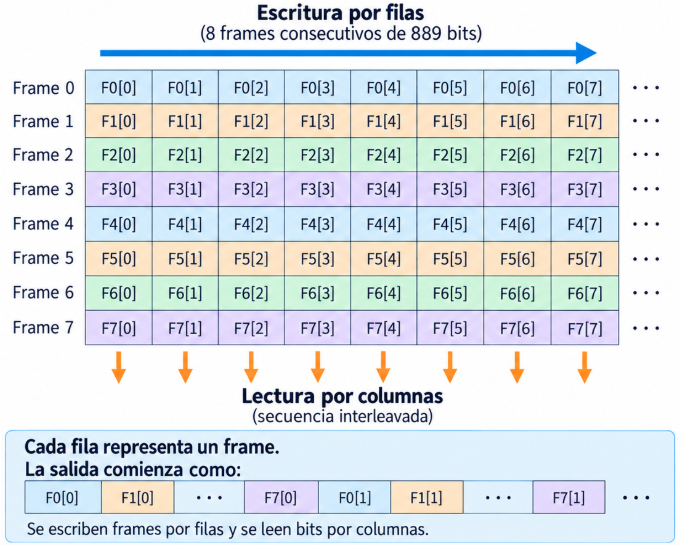
\includegraphics[width=0.65\textwidth]{interleaver_block.png}
    \caption{Interleaver de bloque equivalente.}
    \label{fig:interleaver-block}
\end{figure}

De esta manera, dos bits consecutivos de un mismo frame quedan separados por
ocho posiciones en la salida. Como la permutación de lanes hace que los bits
de una misma codeword reaparezcan cada siete posiciones dentro de cada frame,
para volver a encontrar simultáneamente un bit perteneciente al mismo frame
y a la misma codeword deben avanzarse siete columnas. Cada columna contiene
ocho bits, por lo que la separación resulta

\begin{equation}
    d_{\mathrm{bloque}}
    =
    7\cdot8
    =
    56\text{ bits}.
\end{equation}

Por lo tanto, este interleaver de bloque propuesto permite obtener una 
separación equivalente a la protección del interleaver convolucional
con siete codewords y ocho ramas. Con un BCH capaz de corregir hasta
$t=2$ errores por codeword, la tercera aparición sobre una misma codeword
puede producirse recién luego de 112 posiciones.

Sin embargo, el costo de esta alternativa es considerablemente mayor en 
términos de almacenamiento. Un banco debe contener los ocho frames completos,

\begin{equation}
    M_{\mathrm{bloque}}
    =
    8\cdot889
    =
    7112\text{ bits}.
\end{equation}

Además, para mantener el throughput continuo mientras se recibe el bloque
siguiente y se transmite el anterior, resulta necesario utilizar una
arquitectura de doble banco o \emph{ping-pong}. Mientras un banco se encuentra
en escritura, el otro se utiliza para lectura, intercambiando sus funciones al
finalizar cada bloque. El almacenamiento requerido por lado resulta entonces

\begin{equation}
    M_{\mathrm{bloque,pp}}
    =
    2\cdot7112
    =
    14224\text{ bits}.
\end{equation}

Por lo tanto, para una separación de errores comparable, el interleaver de
bloque requiere aproximadamente

\begin{equation}
    \frac{14224}{3108}
    \approx
    4.6
\end{equation}

veces más almacenamiento que el interleaver convolucional en el transmisor.

Además del costo de memoria, el interleaver de bloque requiere lógica para
generar las direcciones de lectura y escritura, controlar la conmutación entre
los bancos y seleccionar las posiciones que forman el bus paralelo de salida.
Esta lógica introduce una complejidad adicional respecto del interleaver
convolucional, cuya estructura está formada principalmente por retardos fijos.

Para la arquitectura considerada en este trabajo, el interleaver convolucional
presenta una mejor correspondencia con los requisitos del sistema. El datapath
procesa 889 bits por ciclo FEC de manera continua y opera a una frecuencia
cercana a $900\,\mathrm{MHz}$. Los retardos escalonados permiten obtener una
separación de errores comparable a la del interleaver de bloque analizado,
utilizando aproximadamente 3100 bits de almacenamiento por lado y sin requerir
memorias \emph{ping-pong} ni lógica compleja de direccionamiento. Por estas
razones se selecciona el interleaver convolucional frente a una arquitectura
de bloque.

\subsubsection{Presupuesto de latencia}

El presupuesto de latencia se plantea de manera preliminar, ya que la latencia
final de algunos bloques dependerá de la arquitectura adoptada y del grado
de pipeline necesario para cumplir con las restricciones de timing.

En el caso del encoder y decoder BCH, si bien ambos pueden describirse
funcionalmente mediante lógica combinacional, su implementación requiere
registros de pipeline debido a las restricciones de timing asociadas a la
frecuencia objetivo del dominio FEC. En el encoder, la cantidad de lógica
combinacional esperada es relativamente baja, por lo que se estima una
latencia de un ciclo. En cambio, para el decoder se propone preliminarmente un
pipeline de tres etapas. La primera etapa realiza el cálculo de los síndromes,
la segunda determina el polinomio localizador de errores y la tercera realiza
la corrección de las posiciones detectadas. Por lo tanto, se estima una
latencia de tres ciclos FEC.

La permutación de lanes y su operación inversa no introducen latencia, ya que
se implementan como un reordenamiento puramente combinacional de las señales.
Por su parte, el interleaver y el de-interleaver presentan una latencia conjunta
determinada por la arquitectura. Para $B=8$ y $D=1$, los retardos
complementarios de ambas etapas hacen que todos los bits acumulen exactamente
siete ciclos FEC.

El gearbox introduce aproximadamente un ciclo asociado al rearmado de las 
palabras entre ambos anchos de bus. En la FIFO, la latencia depende de su 
ocupación en régimen, como aproximación se considera una ocupación del orden 
de cuatro palabras, consistente con el nivel de arranque adoptado, 
lo que equivale a aproximadamente cuatro ciclos del dominio DSP por cruce. 

A partir de estas hipótesis, el presupuesto preliminar de latencia se resume en
la Tabla~\ref{tab:presupuesto-latencia}.

\begin{table}[H]
\centering
\begin{tabular}{lccc}
\hline
\textbf{Bloque} &
\textbf{Dominio} &
\textbf{Latencia estimada} &
\textbf{Latencia [ns]} \\
\hline

Encoder BCH
& FEC
& $1T_{\mathrm{FEC}}$
& $1.11$ \\

Permutación de lanes
& FEC
& $0$
& $0$ \\

Interleaver + de-interleaver
& FEC
& $7T_{\mathrm{FEC}}$
& $7.78$ \\

Gearbox TX
& FEC
& $1T_{\mathrm{FEC}}$
& $1.11$ \\

FIFO CDC TX
& DSP
& $4T_{\mathrm{DSP}}$
& $5.12$ \\

FIFO CDC RX
& DSP
& $4T_{\mathrm{DSP}}$
& $5.12$ \\

Gearbox RX
& DSP
& $1T_{\mathrm{DSP}}$
& $1.28$ \\

De-permutación de lanes
& FEC
& $0$
& $0$ \\

Decoder BCH
& FEC
& $3T_{\mathrm{FEC}}$
& $3.33$ \\

\hline
\textbf{Total}
& --
& $12T_{\mathrm{FEC}}+9T_{\mathrm{DSP}}$
& $\mathbf{24.85}$ \\
\hline
\end{tabular}
\caption{Presupuesto preliminar de latencia end-to-end}
\label{tab:presupuesto-latencia}
\end{table}

Para $f_{\mathrm{FEC}}=899.89\,\mathrm{MHz}$ se tiene
$T_{\mathrm{FEC}}\approx1.11\,\mathrm{ns}$, mientras que para
$f_{\mathrm{DSP}}=781.25\,\mathrm{MHz}$ resulta
$T_{\mathrm{DSP}}=1.28\,\mathrm{ns}$. Bajo las hipótesis anteriores, la
latencia end-to-end estimada sin considerar el canal es de
$24.85\,\mathrm{ns}$. Este valor resulta de sumar
$12T_{\mathrm{FEC}}+9T_{\mathrm{DSP}}$ y equivale a aproximadamente
$22.37T_{\mathrm{FEC}}$.

% ---------------------------------------------------------------------------
\subsection{Modelos de referencia}
% ---------------------------------------------------------------------------

\subsubsection{Convenciones de representación}

Con el objetivo de garantizar que los modelos en Python y la posterior
implementación RTL utilicen la misma representación de bits, se adopta una 
convención desde un principio para todas las instancias del sistema.

Para un vector de ancho $W$, la señal RTL se declara como
\texttt{[W-1:0]}. El bit de índice cero es el más antiguo del vector y es el
primero que se transmite:

\begin{equation}
    \text{primer bit transmitido}=v[0].
    \label{eq:convencion-orden-vector}
\end{equation}

La representación polinómica asocia directamente el índice de cada bit con el
grado del término correspondiente.

\begin{equation}
    a(x)=\sum_{i=0}^{W-1}a_i x^i
    \quad \Longleftrightarrow \quad 
    a_i=\texttt{a[i]}
\end{equation}

Por ejemplo,

\begin{equation}
    x^3+x+1
    \quad\longleftrightarrow\quad
    \texttt{0b1011}.
\end{equation}

Esta es también la convención utilizada para los elementos de
$\mathrm{GF}(2^7)$. En particular, con el polinomio primitivo

\begin{equation}
    p(x)=x^7+x^3+1,
\end{equation}

el elemento primitivo se representa como

\begin{equation}
    \alpha=x
    \quad\longleftrightarrow\quad
    \texttt{0b0000010}.
\end{equation}

\pagebreak
Para la codificación BCH se adopta una representación sistemática. Sea el
mensaje de 113 bits

\begin{equation}
    m(x)=\sum_{i=0}^{112}m_i x^i.
\end{equation}

El resto de paridad se calcula como

\begin{equation}
    r(x)=x^{14}m(x)\bmod g(x),
    \label{eq:convencion-resto-bch}
\end{equation}

y la palabra codificada queda definida por

\begin{equation}
    c(x)=x^{14}m(x)+r(x),
    \label{eq:convencion-codeword-bch}
\end{equation}

donde la suma se realiza en $\mathrm{GF}(2)$ y, por lo tanto, corresponde a una
operación XOR. La correspondencia entre el polinomio y el vector de 127 bits es

\begin{equation}
    c_i=
    \begin{cases}
        r_i, & 0\leq i<14,\\
        m_{i-14}, & 14\leq i<127.
    \end{cases}
    \label{eq:convencion-mapeo-codeword}
\end{equation}

En consecuencia, los bits de paridad ocupan
\texttt{codeword[13:0]} y los bits de información ocupan
\texttt{codeword[126:14]}.

\subsubsection{Aritmética de \texorpdfstring{$\mathrm{GF}(2^7)$}{GF(2 elevado a 7)}}

Para realizar las operaciones necesarias sobre campos finitos se desarrolló
en Python un par de clases que implementa la aritmética de $\mathrm{GF}(2^m)$ 
(\texttt{GF2m}) y las operaciones con polinomios (\texttt{GFPoly}) 
cuyos coeficientes pertenecen al campo. Estas clases proporcionan suma, 
multiplicación, potenciación, división, inverso multiplicativo, cuadrado, 
traza y tablas exponencial y logarítmica.

La implementación fue validada mediante una prueba exhaustiva sobre los 128
elementos de $\mathrm{GF}(2^7)$. Se comprobaron las operaciones de suma y
multiplicación, las relaciones entre las tablas exponencial y logarítmica, el
cálculo de potencias e inversos, la división, las propiedades de la traza y la
equivalencia entre las distintas interfaces de representación. Todas las
verificaciones finalizaron correctamente.

Para este trabajo se construyó $\mathrm{GF}(2^7)$ utilizando el polinomio
primitivo

\begin{equation}
    p(x)=x^7+x^3+1.
    \label{eq:polinomio-primitivo-gf27-modelo}
\end{equation}

La tabla completa de elementos del campo, incluyendo su representación como
potencia de $\alpha$, su forma polinómica y su representación binaria, se
presenta en la Tabla~\ref{tab:elementos-gf27} del
Anexo~\ref{anexo:elementos-gf27}.

\subsubsection{Polinomio generador y matriz de codificación}

El polinomio generador se obtuvo algorítmicamente a partir de las clases
ciclotómicas $C_1$ y $C_3$. Para cada clase se construyó el polinomio mínimo
sobre $\mathrm{GF}(2)$ asociado a sus raíces en $\mathrm{GF}(2^7)$ y luego se
multiplicaron ambos factores mediante el modelo polinómico desarrollado en
Python. El resultado fue

\begin{equation}
    g(x)
    =
    x^{14}+x^9+x^8+x^6+x^5+x^4+x^2+x+1,
    \label{eq:generador-bch-127-113-etapa1}
\end{equation}

que coincide con el polinomio derivado durante el dimensionamiento del código.
El grado 14 de $g(x)$ determina los 14 bits de redundancia del
BCH(127,113).

La codificación sistemática define una transformación lineal entre los 113
coeficientes del mensaje y los 14 coeficientes del resto. Esta transformación
se representó mediante la matriz de paridad

\begin{equation}
    P\in\mathrm{GF}(2)^{113\times14},
\end{equation}

tal que, para el mensaje
$\mathbf{m}=[m_0,m_1,\ldots,m_{112}]$, su vector de paridad es

\begin{equation}
    \mathbf{r}=\mathbf{m}P.
    \label{eq:matriz-paridad-bch}
\end{equation}

La matriz $P$ se construyó a partir de la codificación sistemática. Para cada
fila $j$ se consideró el mensaje correspondiente al vector de la base
canónica,

\begin{equation}
    m^{(j)}(x)=x^j,
    \qquad 0\leq j<113,
\end{equation}

y se calculó su resto mediante

\begin{equation}
    r^{(j)}(x)
    =
    x^{14}m^{(j)}(x)\bmod g(x).
\end{equation}

Los 14 coeficientes de $r^{(j)}(x)$ forman la fila $j$ de $P$. Por
linealidad, la paridad de un mensaje arbitrario se obtiene como la combinación
XOR de las filas correspondientes a sus bits activos

\begin{equation}
    r_i
    =
    \bigoplus_{j=0}^{112} m_jP_{j,i},
    \qquad 0\leq i<14.
    \label{eq:ecuacion-paridad-paralela}
\end{equation}

La misma transformación puede expresarse mediante la matriz transpuesta

\begin{equation}
    P_{\mathrm{T}}=P^{\mathrm{T}}
    \in\mathrm{GF}(2)^{14\times113}.
\end{equation}

La fila $i$ de $P_{\mathrm{T}}$ contiene los 113 coeficientes del mensaje que
contribuyen al coeficiente de paridad $r_i$. La matriz transpuesta completa se
presenta en la Tabla~\ref{tab:matriz-paridad-bch} del
Anexo~\ref{anexo:matriz-paridad-bch}.

El modelo matricial se comparó contra la codificación sistemática por división 
polinómica utilizando el mensaje nulo, el mensaje con todos sus bits en uno, 
los 113 vectores de la base canónica y 1000 mensajes aleatorios. En todos los 
casos se obtuvo la misma palabra codificada mediante ambos métodos y resto nulo 
al dividir el resultado por $g(x)$.

\subsubsection{Codificación y decodificación BCH}

\paragraph{Codificador.}
La codificación sistemática se realiza mediante la matriz de paridad obtenida
en la sección anterior. Para el mensaje
$\mathbf{m}=[m_0,m_1,\ldots,m_{112}]$, los 14 coeficientes de paridad se
calculan como

\begin{equation}
    \mathbf{r}=\mathbf{m}P,
    \qquad
    \mathbf{r}=[r_0,r_1,\ldots,r_{13}].
    \label{eq:paridad-matricial-codificador}
\end{equation}

El vector $\mathbf{r}$ representa los coeficientes del resto $r(x)$ definido
en la Ecuación~\eqref{eq:convencion-resto-bch}. La palabra codificada se forma
desplazando el mensaje 14 posiciones e insertando la paridad en los términos
de menor grado:

\begin{equation}
    c(x)=x^{14}m(x)+r(x).
    \label{eq:codeword}
\end{equation}

Con el orden creciente de grado adoptado, el vector de coeficientes de la
palabra codificada es

\begin{equation}
    \mathbf{c}
    =
    [c_0,c_1,\ldots,c_{126}]
    =
    [r_0,r_1,\ldots,r_{13},m_0,m_1,\ldots,m_{112}].
    \label{eq:formacion-codeword}
\end{equation}

Así, $c_i=r_i$ para $0\leq i<14$ y $c_i=m_{i-14}$ para
$14\leq i<127$. Por lo tanto, la codificación queda completamente definida por
la transformación lineal $\mathbf{r}=\mathbf{m}P$ y por la inserción de sus 14
coeficientes en los términos de menor grado de $c(x)$.

\paragraph{Decodificador.}
La decodificación del código BCH, con capacidad de corrección $t=2$, se
realiza mediante el algoritmo \textit{search-less} propuesto por Yoo y
Park~\cite{yoo2014}. A diferencia de una búsqueda de Chien, en la que las
raíces del polinomio localizador se determinan evaluándolo sobre las posibles
posiciones de la palabra de código, este método aprovecha que para $t=2$ el
polinomio localizador es cuadrático y puede resolverse algebraicamente.

Sea la palabra recibida

\begin{equation}
    y(x)=c(x)+e(x),
\end{equation}

donde $c(x)$ es una palabra de código válida y $e(x)$ representa el patrón de
errores. Los síndromes se obtienen evaluando la palabra recibida en las raíces
del código BCH:

\begin{equation}
    S_i=y(\alpha^i)
    =
    y_0+y_1\alpha^i+\cdots+y_{n-1}\alpha^{(n-1)i},
\end{equation}

donde $\alpha$ es un elemento primitivo de $\mathrm{GF}(2^m)$. Como
$c(\alpha^i)=0$ para las raíces utilizadas en la construcción del código,

\begin{equation}
    S_i=e(\alpha^i).
\end{equation}

Para un BCH binario con $t=2$ es suficiente trabajar con los síndromes impares
$S_1$ y $S_3$, ya que los síndromes pares pueden obtenerse a partir de ellos
mediante la característica de Frobenius.

El algoritmo distingue los casos de cero, uno y dos errores antes de
resolver el polinomio localizador:

\begin{itemize}
    \item Si $S_1=0$, entonces, bajo la hipótesis de hasta dos errores,
    $S_3=0$ y la palabra se considera libre de errores.

    \item Si $S_1\neq0$ y $S_1^3=S_3$, existe un único error. En este caso
    $\sigma(x)=1+S_1x$, su raíz es $x_1=S_1^{-1}$ y la posición del error es
    $j_1=-\log_{\alpha}(x_1)\bmod127$.

    \item En caso contrario, se considera que existen dos errores y se aplica
    la solución cuadrática \textit{search-less}.
\end{itemize}

La Fig.~\ref{fig:searchless-flow} resume esta secuencia de decisión y las
operaciones efectuadas en cada caso.

\begin{figure}[H]
    \centering
    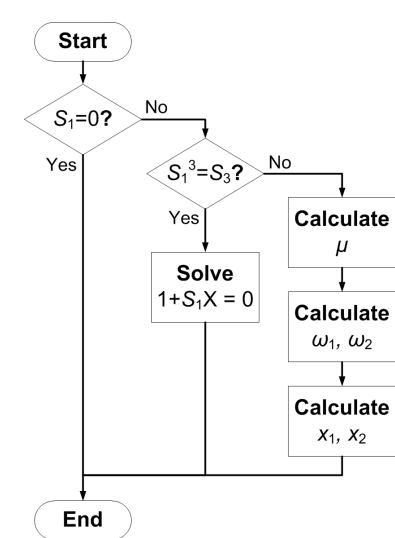
\includegraphics[width=0.34\linewidth]{search-less.png}
    \caption{Flujo del algoritmo de decodificación \textit{search-less} para
    un BCH con $t=2$, adaptado de~\cite{yoo2014}.}
    \label{fig:searchless-flow}
\end{figure}

Para el caso de dos errores, el polinomio localizador puede expresarse como

\begin{equation}
    \sigma(x)=1+\sigma_1x+\sigma_2x^2,
    \label{eq:bch-locator-t2}
\end{equation}

con

\begin{equation}
    \sigma_1=S_1,
    \qquad
    \sigma_2=\frac{S_1^3+S_3}{S_1}.
    \label{eq:sigma}
\end{equation}

El algoritmo \textit{search-less} transforma la búsqueda de las raíces
de~\eqref{eq:bch-locator-t2} en la resolución de una ecuación cuadrática
estándar. Para ello se definen

\begin{equation}
    \omega
    =
    \frac{S_1^3+S_3}{S_1^2}x,
    \qquad
    \mu
    =
    \frac{S_1^3+S_3}{S_1^3}.
    \label{eq:bch-omega-mu}
\end{equation}

Sustituyendo estas expresiones en \eqref{eq:bch-locator-t2}, se obtiene

\begin{equation}
    1+\frac{\omega}{\mu}
      +\frac{\omega^2}{\mu}=0,
\end{equation}

y, multiplicando por $\mu$,

\begin{equation}
    \omega^2+\omega=\mu.
    \label{eq:bch-quadratic}
\end{equation}

De esta manera, la determinación de las dos raíces del polinomio localizador
se reduce a resolver una única ecuación sobre $\mathrm{GF}(2^7)$.

La resolución de \eqref{eq:bch-quadratic} se basa en la traza absoluta de
$\mathrm{GF}(2^m)$ sobre $\mathrm{GF}(2)$, definida como

\begin{equation}
    \operatorname{Tr}(a)
    =
    \sum_{k=0}^{m-1}a^{2^k}.
\end{equation}

La ecuación $\omega^2+\omega=\mu$ posee soluciones en
$\mathrm{GF}(2^m)$ si y sólo si $\operatorname{Tr}(\mu)=0$.
Para obtener directamente una de estas soluciones, el algoritmo selecciona
previamente un elemento $\theta\in\mathrm{GF}(2^m)$ que satisfaga 
$\operatorname{Tr}(\theta)=1$.

En este diseño $m=7$ es impar y, por lo tanto,
$\operatorname{Tr}(1)=m\bmod2=1$. Se adopta entonces la constante
$\theta=1$, que es la misma utilizada por el modelo de referencia y evita
tener que buscar otro elemento del campo durante la decodificación.

Una de las soluciones de \eqref{eq:bch-quadratic} se obtiene como

\begin{equation}
\begin{split}
    \omega_1 ={}&
    \mu\theta^2
    +(\mu+\mu^2)\theta^{2^2}
    +(\mu+\mu^2+\mu^{2^2})\theta^{2^3}
    +\cdots \\
    &+
    \left(
        \mu+\mu^2+\cdots+\mu^{2^{m-2}}
    \right)\theta^{2^{m-1}},
\end{split}
\label{eq:bch-omega1-searchless}
\end{equation}

mientras que la segunda solución se obtiene directamente como

\begin{equation}
    \omega_2=\omega_1+1.
\end{equation}

Finalmente, deshaciendo el cambio de variable definido en
\eqref{eq:bch-omega-mu}, las raíces del polinomio localizador resultan

\begin{equation}
    x_i
    =
    \frac{S_1^2}{S_1^3+S_3}\omega_i
    =
    \frac{\omega_i}{\mu S_1},
    \qquad i\in\{1,2\}.
\end{equation}

A partir de cada raíz se obtiene la posición del error mediante el logaritmo
discreto respecto de $\alpha$,

\begin{equation}
    j_i
    =
    -\log_{\alpha}(x_i)\bmod 127.
\end{equation}

El modelo de referencia en Python se verificó codificando 1000 mensajes
aleatorios y comprobando que las palabras válidas produjeran $S_1=S_3=0$ y
que el decodificador no las modificara. Además, para una palabra válida se
recorrieron exhaustivamente las 127 posiciones posibles de un único error y
las $\binom{127}{2}=8001$ combinaciones posibles de dos errores. En todos los
casos se recuperó la palabra codificada original y los síndromes posteriores
a la corrección fueron nulos.

\paragraph{Comparación con una búsqueda de Chien paralela.}
Una alternativa convencional para localizar los errores consiste en realizar
una búsqueda de Chien, evaluando el polinomio localizador
$\sigma(x)$ sobre los 127 elementos asociados a las posibles posiciones de la
palabra de código. Si se desea realizar la localización completa en un único
ciclo, deben efectuarse las 127 evaluaciones en paralelo.

Para $t=2$, el evaluador correspondiente a la posición $i$ calcula

\begin{equation}
    \sigma(\alpha^{i}) = 1 + \sigma_1\alpha^{i} + \sigma_2\alpha^{2i}.
\end{equation}

Como $\alpha^{i}$ y $\alpha^{2i}$ son constantes conocidas para cada
posición, cada evaluador puede implementarse mediante dos multiplicaciones por
constante en $\mathrm{GF}(2^7)$, una red de sumas en el campo y un detector de
cero. La arquitectura completamente paralela replica esta lógica 127 veces,
obteniendo directamente una máscara de error de 127 bits. La estructura
genérica de un evaluador se muestra en la Fig.~\ref{fig:chien-evaluator}.

\begin{figure}[H]
    \centering
    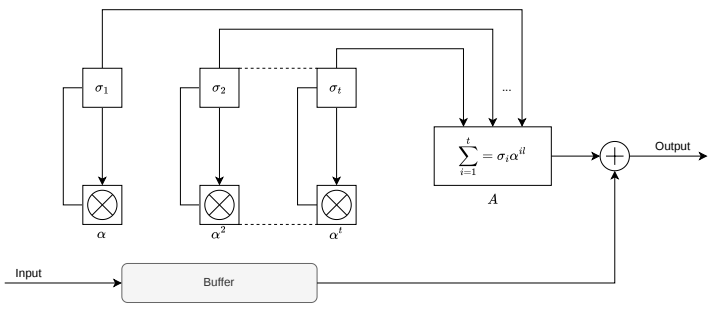
\includegraphics[width=0.65\linewidth]{generic_chien_search.png}
    \caption{Estructura genérica para la evaluación recurrente del polinomio
    localizador en una búsqueda de Chien.}
    \label{fig:chien-evaluator}
\end{figure}

La arquitectura \textit{search-less}, en cambio, reemplaza esta exploración
exhaustiva por un único camino algebraico que obtiene directamente, como
máximo, las dos raíces del polinomio localizador. Su costo se concentra en un
número reducido de operaciones sobre $\mathrm{GF}(2^7)$, principalmente
multiplicaciones, divisiones, cuadrados y conversiones logarítmicas. Su 
estructura se puede visualizar en la Fig.~\ref{fig:search-less-calculator}

\begin{figure}[H]
    \centering
    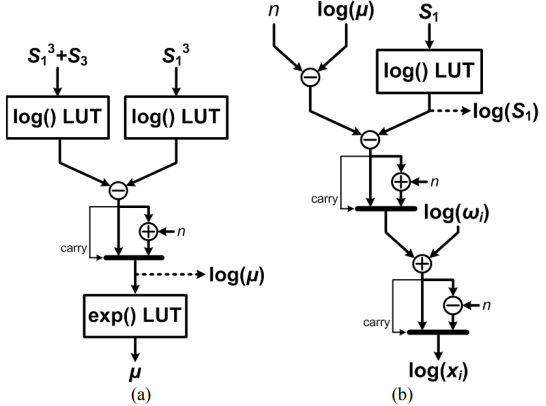
\includegraphics[width=0.5\linewidth]{search-less_calculator.png}
    \caption{Estructura para el calculo de $\mu$ y las raices del polinomio
    localizador de error.}
    \label{fig:search-less-calculator}
\end{figure}

Al no
replicar un evaluador por cada posición del codeword, su área no escala
directamente con $n$ como ocurre en una implementación de Chien completamente
paralela.

El precio de esta reducción de paralelismo espacial es un camino algebraico
más profundo, por lo que la arquitectura \textit{search-less} puede requerir
segmentación mediante registros de pipeline para alcanzar la frecuencia
objetivo. La comparación conceptual entre ambas alternativas se resume en la
Tabla~\ref{tab:comparacion-decoders-bch}.

\begin{table}[H]
    \centering
    \begin{tabular}{@{}p{0.25\linewidth}p{0.32\linewidth}p{0.32\linewidth}@{}}
        \toprule
        \textbf{Característica} &
        \textbf{Chien paralelo} &
        \textbf{Decoder \textit{search-less}} \\
        \midrule

        Localización &
        Evalúa simultáneamente las 127 posiciones &
        Calcula algebraicamente hasta dos raíces \\

        Paralelismo principal &
        127 evaluadores de $\sigma(\alpha^i)$ &
        Un solucionador cuadrático en $\mathrm{GF}(2^7)$ \\

        Operaciones principales &
        Multiplicaciones GF por constantes, XOR y detección de cero &
        Multiplicaciones, cuadrados, división y LUT log/exp \\

        Escalamiento de área &
        Aproximadamente proporcional a $n$ para paralelismo completo &
        Determinado principalmente por la aritmética de campo para $t=2$ \\

        Estructura &
        Muy regular y altamente replicada &
        Menos replicada, con operadores de campo más complejos \\

        Camino combinacional &
        Relativamente corto por evaluador &
        Mayor profundidad algebraica; admite pipeline \\

        Resultado &
        Máscara de error de 127 bits directamente &
        Hasta dos índices, posteriormente convertidos en una máscara \\
        \bottomrule
    \end{tabular}

    \caption{Comparación arquitectónica entre una búsqueda de Chien totalmente
    paralela y el algoritmo \textit{search-less} seleccionado.}
    \label{tab:comparacion-decoders-bch}
\end{table}

Como referencia, Yoo y Park sintetizaron ambas alternativas para un código
BCH(44,32,2) en una tecnología CMOS de 65 nm y el algoritmo \textit{search-less}
presentó una reducción de aproximadamente $50{,}5\%$ en el conteo de compuertas
para una latencia prácticamente equivalente~\cite{yoo2014}.

Estos valores no pueden extrapolarse directamente al BCH(127,113), ya que
cambian tanto la longitud del código como la extensión del campo. Sin embargo,
muestran la ventaja arquitectónica de reemplazar la búsqueda explícita de
raíces por su resolución algebraica.

\subsubsection{Generador PRBS31 paralelo}
\pendiente{Documentar la potenciación de la matriz de transición y su validación contra el modelo serie.}

\subsubsection{Permutación de lanes e interleaver convolucional}
\pendiente{Documentar ambos modelos, sus inversas y la latencia uniforme.}

\subsubsection{Modelo de canal}
\pendiente{Documentar el canal BSC y el generador parametrizable de ráfagas.}

\subsubsection{Autotests y barridos de BER}
\pendiente{Documentar cobertura de casos, semillas y resultados de la cadena completa.}

% ---------------------------------------------------------------------------
\subsection{RTL del transmisor}
% ---------------------------------------------------------------------------

\subsubsection{Generador PRBS31}
\pendiente{Documentar arquitectura paralela y reset.}

\subsubsection{Banco de codificadores BCH}
\pendiente{Documentar la arquitectura de los siete codificadores.}

\subsubsection{Permutación de lanes}
\pendiente{Documentar el mapeo de índices implementado en RTL.}

\subsubsection{Interleaver convolucional}
\pendiente{Documentar parametrización y registros.}

\subsubsection{Gearbox y FIFO CDC}
\pendiente{Documentar la implementación RTL y el mecanismo de arranque.}

% ---------------------------------------------------------------------------
\subsection{RTL del receptor}
% ---------------------------------------------------------------------------

\subsubsection{FIFO CDC y gearbox inverso}
\pendiente{Documentar el retorno al ancho de 889 bits.}

\subsubsection{De-interleaver y de-permutación}
\pendiente{Documentar las transformaciones inversas y su alineamiento.}

\subsubsection{Banco de decodificadores BCH}
\pendiente{Documentar síndromes, localizador cuadrático y corrección.}

\subsubsection{Checker PRBS31 y medición de BER}
\pendiente{Documentar los contadores pre-FEC y post-FEC.}

% ---------------------------------------------------------------------------
\subsection{Verificación en SystemVerilog}
% ---------------------------------------------------------------------------

\subsubsection{Transacciones y generación de estímulos}
\pendiente{Documentar transacciones, semillas, tasa de error y ráfagas.}

\subsubsection{Drivers y monitores}
\pendiente{Documentar las interfaces y el seguimiento de las transacciones.}

\subsubsection{Scoreboard}
\pendiente{Documentar los modos basados en vectores Python y modelo C mediante DPI-C.}

\subsubsection{Cobertura funcional y de código}
\pendiente{Documentar el modelo de cobertura y los resultados alcanzados.}

\subsubsection{Suite de regresión}
\pendiente{Documentar tests dirigidos, aleatorios y resultados por semilla.}

% ---------------------------------------------------------------------------
\subsection{Síntesis lógica}
% ---------------------------------------------------------------------------

\subsubsection{Scripts y restricciones}
\pendiente{Documentar clocks, entradas, salidas, excepciones y restricciones CDC.}

\subsubsection{Timing, área y potencia}
\pendiente{Incorporar y analizar los reportes de Design Compiler.}

\subsubsection{Análisis del camino crítico}
\pendiente{Identificar el bloque limitante y discutir las alternativas de optimización.}

% ---------------------------------------------------------------------------
\subsection{Implementación y medición en FPGA}
% ---------------------------------------------------------------------------

\subsubsection{Clocking y wrapper de integración}
\pendiente{Documentar la generación de ambos clocks a frecuencia reducida.}

\subsubsection{Canal de ruido y generador de ráfagas}
\pendiente{Documentar la implementación configurable en fabric.}

\subsubsection{Interfaz de control}
\pendiente{Documentar la configuración y lectura de contadores desde el PS.}

\subsubsection{Utilización y cierre de timing}
\pendiente{Incorporar los reportes de Vivado.}

\subsubsection{Curvas de BER}
\pendiente{Documentar las mediciones pre-FEC, post-FEC y los barridos de ráfagas.}

% ---------------------------------------------------------------------------
\section{Conclusiones}
% ---------------------------------------------------------------------------

\pendiente{Redactar las conclusiones una vez cerradas las siete etapas.}

\begin{thebibliography}{9}

\bibitem{yoo2014}
I. Yoo e I.-C. Park,
``A Search-less DEC BCH Decoder for Low-Complexity Fault-Tolerant Systems'',
\textit{2014 IEEE Workshop on Signal Processing Systems (SiPS)},
pp.~44--49, 2014.
\href{https://doi.org/10.1109/SiPS.2014.6986060}{doi:10.1109/SiPS.2014.6986060}.

\end{thebibliography}

\clearpage
\appendix

% ---------------------------------------------------------------------------
\section{Elementos de \texorpdfstring{$\mathrm{GF}(2^7)$}{GF(2 elevado a 7)}}
\label{anexo:elementos-gf27}
% ---------------------------------------------------------------------------

El campo se genera con el polinomio primitivo $p(x)=x^7+x^3+1$. Cada vector
$b_6b_5\ldots b_0$ representa el polinomio
$b_6x^6+b_5x^5+\cdots+b_1x+b_0$. La tabla fue obtenida con el modelo
\texttt{GF2m} utilizado para diseñar el código BCH.

\begingroup
\footnotesize
\renewcommand{\arraystretch}{0.92}
\setlength{\LTpre}{0.5em}
\setlength{\LTpost}{0pt}
\begin{longtable}{@{}c l c@{}}
    \caption{Elementos de $\mathrm{GF}(2^7)$ generado por $x^7+x^3+1$.}
    \label{tab:elementos-gf27} \\
    \toprule
    Potencia & Representación polinómica & Representación vectorial \\
    \midrule
    \endfirsthead

    \multicolumn{3}{c}{\tablename~\thetable\ (continuación)} \\
    \toprule
    Potencia & Representación polinómica & Representación vectorial \\
    \midrule
    \endhead

    \midrule
    \multicolumn{3}{r}{Continúa en la página siguiente} \\
    \endfoot

    \bottomrule
    \endlastfoot

    -- & $0$ & \texttt{0000000} \\
    $\alpha^{0}$ & $1$ & \texttt{0000001} \\
    $\alpha^{1}$ & $x$ & \texttt{0000010} \\
    $\alpha^{2}$ & $x^{2}$ & \texttt{0000100} \\
    $\alpha^{3}$ & $x^{3}$ & \texttt{0001000} \\
    $\alpha^{4}$ & $x^{4}$ & \texttt{0010000} \\
    $\alpha^{5}$ & $x^{5}$ & \texttt{0100000} \\
    $\alpha^{6}$ & $x^{6}$ & \texttt{1000000} \\
    $\alpha^{7}$ & $x^{3}+1$ & \texttt{0001001} \\
    $\alpha^{8}$ & $x^{4}+x$ & \texttt{0010010} \\
    $\alpha^{9}$ & $x^{5}+x^{2}$ & \texttt{0100100} \\
    $\alpha^{10}$ & $x^{6}+x^{3}$ & \texttt{1001000} \\
    $\alpha^{11}$ & $x^{4}+x^{3}+1$ & \texttt{0011001} \\
    $\alpha^{12}$ & $x^{5}+x^{4}+x$ & \texttt{0110010} \\
    $\alpha^{13}$ & $x^{6}+x^{5}+x^{2}$ & \texttt{1100100} \\
    $\alpha^{14}$ & $x^{6}+1$ & \texttt{1000001} \\
    $\alpha^{15}$ & $x^{3}+x+1$ & \texttt{0001011} \\
    $\alpha^{16}$ & $x^{4}+x^{2}+x$ & \texttt{0010110} \\
    $\alpha^{17}$ & $x^{5}+x^{3}+x^{2}$ & \texttt{0101100} \\
    $\alpha^{18}$ & $x^{6}+x^{4}+x^{3}$ & \texttt{1011000} \\
    $\alpha^{19}$ & $x^{5}+x^{4}+x^{3}+1$ & \texttt{0111001} \\
    $\alpha^{20}$ & $x^{6}+x^{5}+x^{4}+x$ & \texttt{1110010} \\
    $\alpha^{21}$ & $x^{6}+x^{5}+x^{3}+x^{2}+1$ & \texttt{1101101} \\
    $\alpha^{22}$ & $x^{6}+x^{4}+x+1$ & \texttt{1010011} \\
    $\alpha^{23}$ & $x^{5}+x^{3}+x^{2}+x+1$ & \texttt{0101111} \\
    $\alpha^{24}$ & $x^{6}+x^{4}+x^{3}+x^{2}+x$ & \texttt{1011110} \\
    $\alpha^{25}$ & $x^{5}+x^{4}+x^{2}+1$ & \texttt{0110101} \\
    $\alpha^{26}$ & $x^{6}+x^{5}+x^{3}+x$ & \texttt{1101010} \\
    $\alpha^{27}$ & $x^{6}+x^{4}+x^{3}+x^{2}+1$ & \texttt{1011101} \\
    $\alpha^{28}$ & $x^{5}+x^{4}+x+1$ & \texttt{0110011} \\
    $\alpha^{29}$ & $x^{6}+x^{5}+x^{2}+x$ & \texttt{1100110} \\
    $\alpha^{30}$ & $x^{6}+x^{2}+1$ & \texttt{1000101} \\
    $\alpha^{31}$ & $x+1$ & \texttt{0000011} \\
    $\alpha^{32}$ & $x^{2}+x$ & \texttt{0000110} \\
    $\alpha^{33}$ & $x^{3}+x^{2}$ & \texttt{0001100} \\
    $\alpha^{34}$ & $x^{4}+x^{3}$ & \texttt{0011000} \\
    $\alpha^{35}$ & $x^{5}+x^{4}$ & \texttt{0110000} \\
    $\alpha^{36}$ & $x^{6}+x^{5}$ & \texttt{1100000} \\
    $\alpha^{37}$ & $x^{6}+x^{3}+1$ & \texttt{1001001} \\
    $\alpha^{38}$ & $x^{4}+x^{3}+x+1$ & \texttt{0011011} \\
    $\alpha^{39}$ & $x^{5}+x^{4}+x^{2}+x$ & \texttt{0110110} \\
    $\alpha^{40}$ & $x^{6}+x^{5}+x^{3}+x^{2}$ & \texttt{1101100} \\
    $\alpha^{41}$ & $x^{6}+x^{4}+1$ & \texttt{1010001} \\
    $\alpha^{42}$ & $x^{5}+x^{3}+x+1$ & \texttt{0101011} \\
    $\alpha^{43}$ & $x^{6}+x^{4}+x^{2}+x$ & \texttt{1010110} \\
    $\alpha^{44}$ & $x^{5}+x^{2}+1$ & \texttt{0100101} \\
    $\alpha^{45}$ & $x^{6}+x^{3}+x$ & \texttt{1001010} \\
    $\alpha^{46}$ & $x^{4}+x^{3}+x^{2}+1$ & \texttt{0011101} \\
    $\alpha^{47}$ & $x^{5}+x^{4}+x^{3}+x$ & \texttt{0111010} \\
    $\alpha^{48}$ & $x^{6}+x^{5}+x^{4}+x^{2}$ & \texttt{1110100} \\
    $\alpha^{49}$ & $x^{6}+x^{5}+1$ & \texttt{1100001} \\
    $\alpha^{50}$ & $x^{6}+x^{3}+x+1$ & \texttt{1001011} \\
    $\alpha^{51}$ & $x^{4}+x^{3}+x^{2}+x+1$ & \texttt{0011111} \\
    $\alpha^{52}$ & $x^{5}+x^{4}+x^{3}+x^{2}+x$ & \texttt{0111110} \\
    $\alpha^{53}$ & $x^{6}+x^{5}+x^{4}+x^{3}+x^{2}$ & \texttt{1111100} \\
    $\alpha^{54}$ & $x^{6}+x^{5}+x^{4}+1$ & \texttt{1110001} \\
    $\alpha^{55}$ & $x^{6}+x^{5}+x^{3}+x+1$ & \texttt{1101011} \\
    $\alpha^{56}$ & $x^{6}+x^{4}+x^{3}+x^{2}+x+1$ & \texttt{1011111} \\
    $\alpha^{57}$ & $x^{5}+x^{4}+x^{2}+x+1$ & \texttt{0110111} \\
    $\alpha^{58}$ & $x^{6}+x^{5}+x^{3}+x^{2}+x$ & \texttt{1101110} \\
    $\alpha^{59}$ & $x^{6}+x^{4}+x^{2}+1$ & \texttt{1010101} \\
    $\alpha^{60}$ & $x^{5}+x+1$ & \texttt{0100011} \\
    $\alpha^{61}$ & $x^{6}+x^{2}+x$ & \texttt{1000110} \\
    $\alpha^{62}$ & $x^{2}+1$ & \texttt{0000101} \\
    $\alpha^{63}$ & $x^{3}+x$ & \texttt{0001010} \\
    $\alpha^{64}$ & $x^{4}+x^{2}$ & \texttt{0010100} \\
    $\alpha^{65}$ & $x^{5}+x^{3}$ & \texttt{0101000} \\
    $\alpha^{66}$ & $x^{6}+x^{4}$ & \texttt{1010000} \\
    $\alpha^{67}$ & $x^{5}+x^{3}+1$ & \texttt{0101001} \\
    $\alpha^{68}$ & $x^{6}+x^{4}+x$ & \texttt{1010010} \\
    $\alpha^{69}$ & $x^{5}+x^{3}+x^{2}+1$ & \texttt{0101101} \\
    $\alpha^{70}$ & $x^{6}+x^{4}+x^{3}+x$ & \texttt{1011010} \\
    $\alpha^{71}$ & $x^{5}+x^{4}+x^{3}+x^{2}+1$ & \texttt{0111101} \\
    $\alpha^{72}$ & $x^{6}+x^{5}+x^{4}+x^{3}+x$ & \texttt{1111010} \\
    $\alpha^{73}$ & $x^{6}+x^{5}+x^{4}+x^{3}+x^{2}+1$ & \texttt{1111101} \\
    $\alpha^{74}$ & $x^{6}+x^{5}+x^{4}+x+1$ & \texttt{1110011} \\
    $\alpha^{75}$ & $x^{6}+x^{5}+x^{3}+x^{2}+x+1$ & \texttt{1101111} \\
    $\alpha^{76}$ & $x^{6}+x^{4}+x^{2}+x+1$ & \texttt{1010111} \\
    $\alpha^{77}$ & $x^{5}+x^{2}+x+1$ & \texttt{0100111} \\
    $\alpha^{78}$ & $x^{6}+x^{3}+x^{2}+x$ & \texttt{1001110} \\
    $\alpha^{79}$ & $x^{4}+x^{2}+1$ & \texttt{0010101} \\
    $\alpha^{80}$ & $x^{5}+x^{3}+x$ & \texttt{0101010} \\
    $\alpha^{81}$ & $x^{6}+x^{4}+x^{2}$ & \texttt{1010100} \\
    $\alpha^{82}$ & $x^{5}+1$ & \texttt{0100001} \\
    $\alpha^{83}$ & $x^{6}+x$ & \texttt{1000010} \\
    $\alpha^{84}$ & $x^{3}+x^{2}+1$ & \texttt{0001101} \\
    $\alpha^{85}$ & $x^{4}+x^{3}+x$ & \texttt{0011010} \\
    $\alpha^{86}$ & $x^{5}+x^{4}+x^{2}$ & \texttt{0110100} \\
    $\alpha^{87}$ & $x^{6}+x^{5}+x^{3}$ & \texttt{1101000} \\
    $\alpha^{88}$ & $x^{6}+x^{4}+x^{3}+1$ & \texttt{1011001} \\
    $\alpha^{89}$ & $x^{5}+x^{4}+x^{3}+x+1$ & \texttt{0111011} \\
    $\alpha^{90}$ & $x^{6}+x^{5}+x^{4}+x^{2}+x$ & \texttt{1110110} \\
    $\alpha^{91}$ & $x^{6}+x^{5}+x^{2}+1$ & \texttt{1100101} \\
    $\alpha^{92}$ & $x^{6}+x+1$ & \texttt{1000011} \\
    $\alpha^{93}$ & $x^{3}+x^{2}+x+1$ & \texttt{0001111} \\
    $\alpha^{94}$ & $x^{4}+x^{3}+x^{2}+x$ & \texttt{0011110} \\
    $\alpha^{95}$ & $x^{5}+x^{4}+x^{3}+x^{2}$ & \texttt{0111100} \\
    $\alpha^{96}$ & $x^{6}+x^{5}+x^{4}+x^{3}$ & \texttt{1111000} \\
    $\alpha^{97}$ & $x^{6}+x^{5}+x^{4}+x^{3}+1$ & \texttt{1111001} \\
    $\alpha^{98}$ & $x^{6}+x^{5}+x^{4}+x^{3}+x+1$ & \texttt{1111011} \\
    $\alpha^{99}$ & $x^{6}+x^{5}+x^{4}+x^{3}+x^{2}+x+1$ & \texttt{1111111} \\
    $\alpha^{100}$ & $x^{6}+x^{5}+x^{4}+x^{2}+x+1$ & \texttt{1110111} \\
    $\alpha^{101}$ & $x^{6}+x^{5}+x^{2}+x+1$ & \texttt{1100111} \\
    $\alpha^{102}$ & $x^{6}+x^{2}+x+1$ & \texttt{1000111} \\
    $\alpha^{103}$ & $x^{2}+x+1$ & \texttt{0000111} \\
    $\alpha^{104}$ & $x^{3}+x^{2}+x$ & \texttt{0001110} \\
    $\alpha^{105}$ & $x^{4}+x^{3}+x^{2}$ & \texttt{0011100} \\
    $\alpha^{106}$ & $x^{5}+x^{4}+x^{3}$ & \texttt{0111000} \\
    $\alpha^{107}$ & $x^{6}+x^{5}+x^{4}$ & \texttt{1110000} \\
    $\alpha^{108}$ & $x^{6}+x^{5}+x^{3}+1$ & \texttt{1101001} \\
    $\alpha^{109}$ & $x^{6}+x^{4}+x^{3}+x+1$ & \texttt{1011011} \\
    $\alpha^{110}$ & $x^{5}+x^{4}+x^{3}+x^{2}+x+1$ & \texttt{0111111} \\
    $\alpha^{111}$ & $x^{6}+x^{5}+x^{4}+x^{3}+x^{2}+x$ & \texttt{1111110} \\
    $\alpha^{112}$ & $x^{6}+x^{5}+x^{4}+x^{2}+1$ & \texttt{1110101} \\
    $\alpha^{113}$ & $x^{6}+x^{5}+x+1$ & \texttt{1100011} \\
    $\alpha^{114}$ & $x^{6}+x^{3}+x^{2}+x+1$ & \texttt{1001111} \\
    $\alpha^{115}$ & $x^{4}+x^{2}+x+1$ & \texttt{0010111} \\
    $\alpha^{116}$ & $x^{5}+x^{3}+x^{2}+x$ & \texttt{0101110} \\
    $\alpha^{117}$ & $x^{6}+x^{4}+x^{3}+x^{2}$ & \texttt{1011100} \\
    $\alpha^{118}$ & $x^{5}+x^{4}+1$ & \texttt{0110001} \\
    $\alpha^{119}$ & $x^{6}+x^{5}+x$ & \texttt{1100010} \\
    $\alpha^{120}$ & $x^{6}+x^{3}+x^{2}+1$ & \texttt{1001101} \\
    $\alpha^{121}$ & $x^{4}+x+1$ & \texttt{0010011} \\
    $\alpha^{122}$ & $x^{5}+x^{2}+x$ & \texttt{0100110} \\
    $\alpha^{123}$ & $x^{6}+x^{3}+x^{2}$ & \texttt{1001100} \\
    $\alpha^{124}$ & $x^{4}+1$ & \texttt{0010001} \\
    $\alpha^{125}$ & $x^{5}+x$ & \texttt{0100010} \\
    $\alpha^{126}$ & $x^{6}+x^{2}$ & \texttt{1000100} \\
\end{longtable}
\endgroup

\clearpage
% ---------------------------------------------------------------------------
\section{Matriz de paridad transpuesta del codificador BCH(127,113)}
\label{anexo:matriz-paridad-bch}
% ---------------------------------------------------------------------------

La matriz transpuesta $P_{\mathrm{T}}$ utilizada en RTL tiene 14 filas y 113
columnas. Cada fila \texttt{P\_T[i]} es una máscara de 113 bits cuyos bits
indican qué posiciones del mensaje contribuyen al bit de paridad $r_i$. La
Tabla~\ref{tab:matriz-paridad-bch} presenta estas máscaras en representación
hexadecimal, con los ceros de mayor peso necesarios para conservar su ancho.

\begingroup
\small
\renewcommand{\arraystretch}{1.05}
\setlength{\LTpre}{0.5em}
\setlength{\LTpost}{0pt}
\begin{longtable}{@{}c c@{}}
    \caption{Filas de la matriz transpuesta $P_{\mathrm{T}}$ utilizada en RTL.}
    \label{tab:matriz-paridad-bch} \\
    \toprule
    \textbf{Fila $P_{\mathrm{T}}[i]$} & \textbf{Hexadecimal (113 bits)} \\
    \midrule
    \endfirsthead

    \multicolumn{2}{c}{\tablename~\thetable\ (continuación)} \\
    \toprule
    \textbf{Fila $P_{\mathrm{T}}[i]$} & \textbf{Hexadecimal (113 bits)} \\
    \midrule
    \endhead

    \midrule
    \multicolumn{2}{r}{Continúa en la página siguiente} \\
    \endfoot

    \bottomrule
    \endlastfoot

    0 &  \texttt{0x15BF0314369552A2D78A6784EE361} \\
    1 &  \texttt{0x1EC1053C5BBFF7E7789EA88D325A3} \\
    2 &  \texttt{0x083D096C81EABD6C26B7369E8A827} \\
    3 &  \texttt{0x107A12D903D57AD84D6E6D3D1504E} \\
    4 &  \texttt{0x154B26A6313FA7124D56BDFEC43FD} \\
    5 &  \texttt{0x1F294E5854EA1C864D271C796649B} \\
    6 &  \texttt{0x0BED9FA49F416BAE4DC45F7622A57} \\
    7 &  \texttt{0x17DB3F493E82D75C9B88BEEC454AE} \\
    8 &  \texttt{0x1A097D864B90FC1BE09B1A5C64A3D} \\
    9 &  \texttt{0x01ADF818A1B4AA9516BC533C2771B} \\
    10 & \texttt{0x035BF0314369552A2D78A6784EE36} \\
    11 & \texttt{0x06B7E06286D2AA545AF14CF09DC6C} \\
    12 & \texttt{0x0D6FC0C50DA554A8B5E299E13B8D8} \\
    13 & \texttt{0x1ADF818A1B4AA9516BC533C2771B0} \\
\end{longtable}
\endgroup

\end{document}
